\section{Grundlagen}
\label{sub:grundlagen}
\subsection{Genetische Algorithmen}

Genetische Algorithmen sind eine Klasse von Optimierungsalgorithmen, die sich an den Mechanismen der natürlichen Evolution orientieren (\cite{Simon.2013}).
Namentlich Mutation, Crossover und Selektion.
Die Begrifflichkeiten orientieren sich entsprechen an der natürlichen Evolution.
Genetische Algorithmen arbeiten typischerweise auf Gruppen von Individuen, auch Population genannt.
Diese Populationen entwickeln sich über die Iterationen des Algorithmus, typischerweise Generationen genannt.
Jedes Individuum besitzt einen Genotypen sowie einen Phänotypen.
%\missingfigure{Vllt. Bild geno phäno}
Der Genotyp eines Individuums ist meist ein Vektor, das Genom des Individuums genannt, der aus einzelnen Zahlen, den Genen des Individuums, besteht.
Dieser stellt die genetischen Informationen eines Individuums dar. 
Daneben existiert in genetischen Algorithmen eine Mapping-Funktion mit der ein Genotyp in einen Phänotyp, sprich eine konkrete Lösung des Optimierungsproblems, übersetzt werden kann.

\begin{algorithm}
\caption{Genetischer Algorithmus} \label{alg:geneticAlgorihtm}
\begin{algorithmic}[1]
	\Procedure{GeneticAlgorithm}{$fitnessFunction,hyperparameters$}
	\State $population \gets initializePopulation$
	\State $populationFitness \gets fitnessFunction(population)$
	\For{$numberIterations$}
		\State $children \gets crossover(population,hyperparameters)$
		\State $children \gets mutate(children,hyperparameters)$
		\State $childFitness = fitnessFunction(children)$
		\State $population \gets selection(population,populationFitness,children,childFitness)$
		\State $populationFitness \gets updateFitness(population)$
	\EndFor
	\EndProcedure
\end{algorithmic}
\end{algorithm}

Die Mechanismen der Mutation und des Crossovers agieren auf der Ebene des Genotyps.
Mutation beschreibt die Situation, dass sich jedes Gen zufällig mutieren kann.
Das bedeutet, dass eine Mutationswahrscheinlichkeit existiert, mit der sich jedes Gen ändern kann.
Abhängig vom Typen des Gens, ist eine Änderung unterschiedlich formuliert, eine reelle Zahl mag sich anhand einer Normalverteilten Zufallsvariable ändern, eine natürliche Zahl mit $\pm1$ und ein Index mag einen zufälligen anderen möglichen Index annehmen.
Mutation ist für einen genetischen Algorithmus wichtig, da sich durch diese neue Eigenschaften entwickeln können.

Crossover beschreibt die Situation, dass zwei oder mehr Elternindividuen zu einem Kindindividuum kombiniert werden. 
Auch hier ist eine konkrete Implementierung nicht vorgeschrieben, wichtig ist nur, dass ein Kind als Kreuzung der Eltern erzeugt werden kann.
Das Ziel des Crossovers ist es, dass sich positive Eigenschaften in Populationen verteilen und mehrere unabhängig entstandenen positiven Mutationen in einem Individuum vereint werden.
Es ist allerdings anzumerken, dass Crossover einen optionalen Teil von genetischen Algorithmen darstellt, einige Algorithmen%, wie beispielsweise ($1 + \lambda$)-ES 
verzichten aus verschiedenen Gründen auf Crossover und mutieren ihre Populationen nur.
Diese beiden Methoden stellen sicher, dass erstens neues genetisches Material Einzug in den Algorithmus finden kann, und das sich genetische Informationen über Generationen in Populationen verteilen können.
Dadurch können systematisch neue Genotypen und damit neue Lösungen generiert werden, sie stelle allerdings keinen Mechanismus zur Verfügung, der Lösungen optimieren kann.

Dieser Mechanismus, der der Optimierung eine Richtung gibt, ist die Selektion.
Anders als die ersten beiden agiert diese auf Phänotypen, sprich ausgedrückten Lösungen.
Jeder genetische Algorithmus benötigt eine Funktion mit der Lösungen bewertet werden können.
Dies kann entweder in Form einer Fitnessfunktion, die die Güte eines Individuums berechnet, bei der höhere Werte besser sind, oder in der Form einer Kostenfunktion, die die Kosten eines Individuums berechnet und bei der entsprechend niedrigere Werte besser sind, geschehen.
Ob eine Fitness- oder Kostenfunktion genutzt wird hängt von der Problemformulierung ab und ist letztendlich nur eine Frage der Algorithmus minimiert oder maximiert.
Mit diesen Funktionen kann für jedes Individuum eine Qualität berechnet werden und Individuen können bezüglich dieser verglichen werden.
Durch Selektion werden in jeder Iteration dann schlechte Lösungen eliminiert, wodurch sich die Population zu Optima hin entwickelt.
Häufig ist die Selektion aus verschiedenen Gründen komplexer, als die einfache Auswahl der besten Individuen.
Besonders die Diversität ist eine erwünschte Eigenschaft, die eine andere Formulierung der Selektion benötigt.
Die in \cref{sub:divergentGeneticAlgorithms} besprochenen Ansätze zum Diversitätsmanagement, berücksichtigen Diversität von Populationen , bevorzugen dabei solche Lösungen, die die Diversität aufrechterhalten und produzieren damit am Ende diversere Ergebnisse, als ein evolutionärer Algorithmus ohne solche Ansätze.

Insgesamt lässt sich ein evolutionärer Algorithmus also wie folgt zusammenfassen.
Zuerst wird eine zufällige Startpopulation erzeugt.
Daraufhin werden aus den Individuen dieser Population Kinder per Crossover erzeugt und mutiert.
Für diese Kinder wird die Fitness berechnet und Selektion durchgeführt, wodurch eine neue Population entsteht, die daraufhin zur neuer Elterngeneration wird.
Die Crossover$\rightarrow$Mutation$\rightarrow$Selektion Schleife wird so oft wiederholt werden bis entweder ein Abbruchkriterium, wie eine zu niedrige Verbesserungsrate, oder die maximale Anzahl an Generationen erreicht ist.
Die letzte erzeugte Population stellt dann die Lösungspopulation des Algorithmus dar.

\subsubsection{Divergente genetische Algorithmen}

\label{sub:divergentGeneticAlgorithms}

Eine sehr häufige Anforderung an genetische Algorithmen ist die Einbindung von Divergenz, bzw. Diversität.
Dies hat verschiedene Gründe.
Einerseits führt eine niedrige Diversität der Individuen dazu, dass nur ein kleiner Bereich des Suchraums, nämlich der in dem die Individuen liegen abgesucht wird.
Sehr homogene Populationen können dadurch einfach in lokalen Optima stagnieren, da andere Optima zu weit im Suchraum entfernt sind.
In einer diversen Population ist das Springen aus lokalen Optima hingegen einfacher und selbst wenn Populationen stagnieren, dann geschieht dies in mehreren Optima gleichzeitig, wodurch die Wahrscheinlichkeit ein im globalen Vergleich gutes lokales Optimum zu finden steigt.
Auch ist es nicht unbedingt wünschenswert eine sehr homogene Population als Ergebnis zu erhalten, da die Individuen mit hoher Wahrscheinlichkeit alle der gleichen Lösungsklasse angehören.
Wenn man eine diverse Population aus Individuen erhält, können Aussagen über unterschiedliche Lösungsklassen getroffen werden, Lösungsklassen und ihre Qualität können miteinander verglichen werden, und je nachdem kann größere Erkenntnis erlangt werden, was eine qualitativ hochwertige Lösung ausmacht , wodurch wiederum das gestellte Problem besser verstanden werden kann.

Es existieren verschiedenste Ansätze, um Diversität zu gewährleisten, welche sind grundsätzlich in genotypische und phänotypische Ansätze aufteilen lassen, abhängig davon auf welcher Ebene Diversitätsmanagement stattfindet.
Ansätze wie Niching (\cite{Mahfoud.1996},\cite{Shir.2012}), gewährleisten genotypische Diversität durch die Ermittlung der genetischen Ähnlichkeit zweier Individuen.
Das hat den Vorteil, dass der Genotyp eines Individuums typischerweise ein Vektor ist, und eine Vielzahl von Ähnlichkeits- und Distanzmetriken für Vektoren existiert.
Dadurch fällt die Definition, was Diversität bedeutet sehr leicht.
Auch ist die Berechnung einer Distanz zwischen Vektoren sehr effizient, was vorteilhaft ist, da die Berechnung der Ähnlichkeit zweier Individuen sehr häufig stattfinden muss.
Allerdings hat es den Nachteil, dass, besonders wenn die Genotyp-zu-Phänotyp-Mapping Funktion komplex ist, genetische Distanz nicht funktionaler Distanz zwischen Lösungen entspricht.
Ist das der Fall besteht die Möglichkeit, dass genetische unähnliche Individuen trotzdem zur die gleiche Lösungsklasse gehören können.
Oft ist mit Diversität funktionale Diversität, sprich Distanz der Phänotypen, gemeint, nicht Diversität der Enkodierung.
Deshalb wurden Ansätze wie Novelty-Search (\cite{Lehman.2011}) oder MAP-Elites (\cite{Mouret.4202015}) zum Diversitätsmanagement vorgeschlagen, die Diversität auf der Ebene, des Phänotyps bestimmen und somit funktionale Distanz messen.
Da der Phänotyp domänenspezifisch,  muss die Diversitätsmetrik für jede Domäne maßgeschneidert definiert werden, und es kann nicht auf Allgemeinlösungen zurückgegriffen werden.
Auch besteht eine erhebliche Limitierung bezüglich der Komplexität einer solche Diversitätsmetrik, da die Ähnlichkeit zweier Phänotypen sehr häufig berechnet werden muss.

\subsubsection{MAP-Elites}

\label{sub:mapElites}
\begin{algorithm}
	\caption{MAP-Elites} 
	\label{alg:mapElites}
	\begin{algorithmic}[1]
		\Procedure{MapElites}{$fitnessFunction,categorizationFunction,hyperparameters$}
		\State $map \gets $ \Comment{Initialize empty n-dimensional map}
		\State $fitness \gets $ \Comment{Initialize empty n-dimensional fitnessMap}
		\State $population \gets initializeRandomPopulation$ \Comment{Start of with randomly generated intitial samples}
		\For{$individual in population$}
			\State $f = fitnessFunction(individual)$
			\State $c = categorizationFunction(individual)$ \Comment{Categorization c is an Index to a cell in the map}
			\If{$map(c) = \emptyset \lor f < fitness(c)$} \Comment{If cell is unoccupied or this solution is better put it in cell}
				\State $map(c) \gets individual$
				\State $fitness(c) \gets f$
			\EndIf
		\EndFor
		
		\For{$numberGenerations$}
			\State $children \gets selectRandom(population,childrenPerGeneration)$ \Comment{Select samples randomly from existing solutions}
			\State $children \gets variate(children,hyperparameters)$ \Comment{Variate these children with crossover and/or mutation}
			\For{$individual in children$}
				\State $f = fitnessFunction(individual)$
				\State $c = categorizationFunction(individual)$
				\If{$map(c) = \emptyset \lor f < fitness(c)$}
					\State $map(c) \gets individual$
					\State $fitness(c) \gets f$
				\EndIf
			\EndFor
		\EndFor
		\Return $map,fitness$
		\EndProcedure
	\end{algorithmic}
\end{algorithm}
MAP-Elites (Multi-dimensional Archive of Phenotypic Elites)(\cite{Mouret.4202015}) ist ein genetischer Algorithmus mit phänotypischem Diversitätsmanagement.
Das bedeutet, dass die Morphologie bzw. Funktionalität einer konkreten ausgedrückten Lösung, wie beispielsweise Volumen oder Krümmung eines Bauteils, betrachtet wird.
Dazu wird der Lösungsraum entlang anhand beliebig vieler Features aufgeteilt, deren Untersuchung als zielführend zum Verständnis des Problems befunden wird.
Diese Feature-Dimensionen sind direkte Merkmale der Phänotypen von Lösungen, wie beispielsweise das Volumen eines Phänotyps in einer dreidimensionalen Domäne.
Als Features sollten solche Merkmale gewählt werden, die unabhängig von der Zielfunktion sind, d.~h. deren Einfluss auf die Fitness von Lösungen unklar ist.
Gerade die Untersuchung wie Merkmale mit der Fitness interagieren ist ein typisches Untersuchungsziel bei der Nutzung von MAP-Elites.
Diesen Feature-Dimensionen wird ein Minimum, Maximums sowie eine Schrittweite zugewiesen um den Lösungsraum in Zellen zu diskretisieren.
Diese Diskretisierung zu Zellen wird typischerweise Karte oder Archiv genannt.
Wichtig für MAP-Elites ist, dass jede Zelle nur maximal eine Lösung enthalten kann.

Zu Beginn des Algorithmus werden alle Zellen leer initialisiert, im Laufe des Algorithmus werden diese nach und nach gefüllt.
Zuerst werden zufällige Individuen generiert um die Karte mit einer Initialpopulation zu befüllen.
Daraufhin werden in jeder Generation aus den momentan in der Karte enthaltenen Lösung zufällig Individuen ausgewählt.
Aus dieses ausgewählten Individuen wird eine Kindpopulation per Mutation und/oder Crossover erzeugt.
Jedes dieser Kinder wird bezüglich der Fitness evaluiert und dessen zugehöriger Phänotyp wird nach den gewählten Features kategorisiert.
Diese Kategorisierung weist jedem Kind eine Zelle zu die es befüllen könnte.
Ist diese Zelle noch leer befüllt das Kind diese, befindet sich bereits ein Individuum in der Zelle, findet zwischen diesem und dem Kind lokal Konkurrenz statt.

Die lokale Konkurrenz innerhalb der Zellen ist was MAP-Elites zu einem divergenten Algorithmus macht.
Da Lösungen nur durch Lösungen verdrängt werden können, denen die gleiche Zelle zugewiesen ist, können Lösungen nur durch phänotypisch ähnliche Lösungen ersetzt werden.
Dadurch wird die phänotypische Diversität des Algorithmus gewährleistet.
Außerdem kann die Größe des Archivs während des Algorithmus nur zunehmen, da Individuen nur verdrängt werden können, wenn sie durch ein anderes ersetzt werden, aber im Laufe des Algorithmus immer mehr leere Zellen befüllt werden können.
Dass bedeutet, dass die Anzahl an lokalen Optima, die der Algorithmus ermittelt hat, über dessen Laufzeit wächst.
Nicht nur wird eine Vielzahl von Lösungen generiert, die unterschiedliche Lösungsklassen abdecken, sondern die regelmäßig aufgeteilte Karte kann auch dabei helfen die Effekte, die die Features auf die Lösungsqualität haben zu verstehen.


\subsection{Surrogat-Modellierung}

\label{sub:surrogate}
Für die Selektion von Individuen innerhalb eines genetischen Algorithmus wird die Lösungsqualität dieser Individuen, typischerweise Fitness genannt, benötigt.
Durch die große Anzahl an Individuen, die für den evolutionären Algorithmus benötigt werden, findet die Auswertung der Fitnessfunktion sehr häufig statt.
Dies stellt bei relativ einfachen Fitnessfunktionen keine große Einschränkung dar, auf Problemdomänen in denen die Auswertung der Fitness eines Individuums allerdings komplexer und dadurch zeitaufwändiger wird, kann dies die Anwendbarkeit einfacher genetischer Algorithmen einschränken.

Aerodynamische Probleme, für die zeitaufwändige Simulationen nötig sind, gehören ohne Zweifel zu der Klasse von Problemen, für die die Anzahl der benötigten Funktionsauswertungen zu groß sind, als dass der Algorithmus in vertretbarer Laufzeit abschließen kann.
Um evolutionäre Algorithmen auf eine solche Problemdomäne anzuwenden, wird eine Möglichkeit benötigt, um die Anzahl der benötigten Funktionsauswertungen erheblich zu reduzieren.
Eine solche Möglichkeit ist die Nutzung eines Surrogatmodells (\cite{Jin.2011},\cite{Preen.2016}), eine Machine-Learning Modell, welches aufgrund echter Simulationsauswertungen trainiert wird, um deren Ergebnis annähernd vorherzusagen.
Eine Auswertung des Modells erfordert dabei nur einen winzigen Bruchteil des Aufwands, der für eine Simulation nötig wäre.

Die Einführung eines Surrogatmodells bringt allerdings einige Probleme mit sich.
Das wichtigste zu lösende Problem ist, wie bestimmt wird anhand welcher realen Funktionsauswertungen das Surrogatmodell trainiert wird.
Dabei müssen einige Ziele beachtet werden.
Ersten sollte das Surrogatmodell möglichst präzise sein, da es seinen Zweck für reale Funktionsauswertungen einzustehen nur erfüllen kann, wenn die Vorhersagen des Surrogatmodells ausreichend gut reale Funktionsauswertungen abbilden.
Da das Surrogatmodell aber genau für den Zweck genutzt wird die Anzahl an benötigten teuren Funktionsauswertungen zu reduzieren, wäre es sinnvoll, wenn Funktionsauswertungen so gewählt werde, dass sie maximalen Nutzen bringen.


\subsubsection{Gaußprozesse}
\label{sub:gp}
\begin{figure}[h]
	\centering
	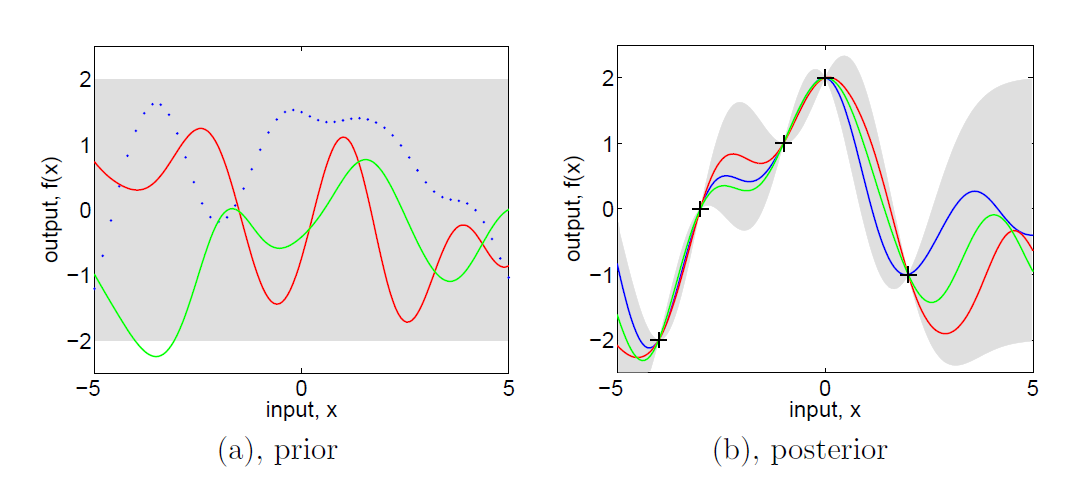
\includegraphics[width=1\linewidth]{bilder/gp}
	\caption{Gaußprozess im Ausgangszustand (a) und nach dem Lernen von fünf Datenpunkten (b) (aus \cite{Rasmussen.2008})}
	\label{fig:gp}
\end{figure}

Gaußprozesse sind ein in \cite{Rasmussen.2008} entwickeltes Machine-Learning Verfahren, mit welchem beliebige mathematische Funktionenen approximiert werden können.
Ein großer Vorteil von Gaußprozessen ist, dass sie durch ihre Herkunft aus der Statistik die zu approximierende Funktion als Wahrscheinlichkeitsverteilung modellieren.
Wie jedes überwachte Machine-Learning Verfahren zur Regression erhalten Gaußprozesse dabei eine Reihe an Beobachtungen auf deren Basis das Modell konstruiert wird.
Vor dem Lernen sind Gaußprozesse als Basisvermutung initialisiert.
Diese Basisvermutung besteht aus eine Mittelwerts- und einer Varianzfunktion, die entsprechend den Mittelwert und Varianz für alle Eingabewerte vorgeben.
Die Funktionen sind frei wählbar, wenn allerdings nichts über das Problem bekannt ist, so wird meist auf konstante Funktionen zurückgegriffen.
In \cref{fig:gp} (a) ist eine solche Basisannahme, mit konstanter Mittelwertfunktion $m(x)=0$ und konstanter Varianzfunktion $v(x)=2$ dargestellt (graues Band).
Außerdem sind 3, der unendlich vielen möglichen Funktionen, die die Daten beschrieben eingezeichnet.

Diese Basisannahme wird daraufhin mit einer Reihe von Beobachtungen trainiert, wodurch sich das in \cref{fig:gp} (b) dargestellte Ergebnis ergibt.
Vom Zustand \cref{fig:gp} (a) zu \cref{fig:gp} (b) wurde der Gaußprozess auf Basis von fünf Datenpunkten trainiert (als $+$-Symbole dargestellt).
An jeder Beobachtung wird der Mittelwert auf den beobachteten Wert gesetzt und die Varianz an dieser Stelle kollabiert zu null, da dort absolute Sicherheit bezüglich des Wertes besteht.
Auch die Varianzen um die Datenpunkte nehmen stark ab, werden allerdings nicht null.
Je näher ein Punkt an tatsächlichen Beobachtungen liegt, desto kleiner ist die Varianz.
Dies ist durch die Grundannahme zu begründen, dass die zu approximierende Funktion als stetig behandelt werden kann, d.~h. es wird angenommen, dass kleine Änderungen der Eingabewerte in kleinen Änderungen der Funktionswerte resultieren.

Gaußprozesse werden primär durch die Wahl der drei innerhalb des Gaußprozesses benötigten Funktionen und deren Hyperparameter gesteuert.
Die Mittelwertsfunktion ist die anfängliche Annahme des Mittelwerts des Gaußprozesses.
Durch diese wird die Grundannahme des Gaußprozesses in Bereichen in denen keine Datenpunkte bekannt sind definiert.
Wie diese Funktion aussehen kann, ist nicht weiter beschränkt, die Daten sollten allerdings durch diese Funktion beschreibbar sein.
Ein linearer Mittelwert kann beispielsweise niemals korrekt durch eine konstante Mittelwertfunktion beschrieben werden.
In \cref{fig:gp} ist ein Beispiel einer konstanten Mittelwertfunktion abgebildet.
Die Hyperparameter der Mittelwertsfunktion hängen stark von der Funktion ab, die hier gewählt wird, im Falle von polynomiellen Funktionen wären dies die Koeffizienten.

Typischerweise wird davon ausgegangen, dass die Eingabedaten, mit denen der Gaußprozess trainiert, wird nicht rauschfrei sind.
Zur Beschreibung des Rauschens des Signals existiert die Wahrscheinlichkeits-Funktion.
Diese Funktion ist eine Wahrscheinlichkeitsverteilung, die das Rauschen beschreibt.
Die typische Annahme ist, dass das Rauschen normalverteilt ist.
Wenn die Wahrscheinlichkeitsfunktion eine Normalverteilung ist, wird diese nur durch $\sigma$ parametrisiert.
In Szenarien in denen eine Normalverteilung zur Beschreibung des Rauschens nicht korrekt ist, müssen stattdessen andere Verteilungen herangezogen werden.
Hyperparameter der Wahrscheinlichkeits-Funktion sind die Hyperparameter der gewählten Verteilung.

Die letzte und wichtigste der Funktionen ist die Kovarianzfunktion.
Die Aufgabe der Kovarianzfunktion ist es die Kovarianz zwischen Punkte zu berechnen.
Damit wird durch die Kovarianzfunktion gesteuert welche Punkte für wie ähnlich befunden werden und damit wie Beobachtungen sich auf ihre Umgebung auswirken.
Der wichtigste Hyperparameter der Kovarianzfunktion ist das Längenmaß $\ell$.
\begin{figure}[h]
	\centering
	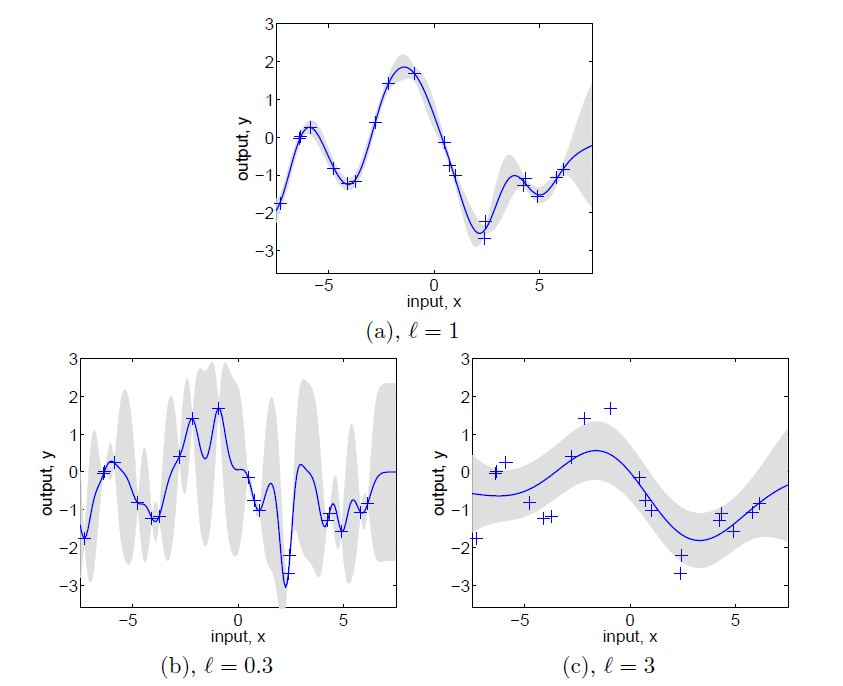
\includegraphics[width=1\linewidth]{bilder/lengthscale}
	\caption{Mittelwert und $2\sigma$-Intervall von Gaußprozessen mit unterschiedlichen Längenmaßen, Beobachtungen sind als "+" dargestellt (aus \cite{Rasmussen.2008})}
	\label{fig:lengthscale}
\end{figure}
Das Längenmaß bestimmt wie weit der Einfluss einer Beobachtung reicht.
Bei kleinen Längenmaßen steigt die Varianz schnell an je weiter man sich von einer Beobachtung wegbewegt, bei größeren Längenmaßen haben Beobachtungen einen weiteren Einfluss und die Funktionen werden glatter.
In \cref{fig:lengthscale} ist ein Gaußprozess mit unterschiedlichen Längenmaßen dargestellt.
Es ist zu Erkennen das \cref{fig:lengthscale} (b) wesentlich steiler ist als \cref{fig:lengthscale} (a \& c).
Auch ist zu Erkennen, dass für $\ell=0.3$ die Varianz schnell ansteigt, wenn man sich von Beobachtungen entfernt.
Im Gegensatz dazu ist in \cref{fig:lengthscale} (c) der Gaußprozess mit $\ell = 3$ dargestellt. 
Dessen Mittelwert ist wesentlich glatter, beschreibt die Punkte aber nicht gut. 
Stattdessen wird für diese höheren Längenmaße ein größeres $\sigma_n$ der Wahrscheinlichkeits-Funktion benötigt. 
Kurz gesagt beschreibt der Gaußprozess mit $\ell=3$ eine glatte Funktion mit starkem Rauschen.
Es sollte klar erkennbar sein, dass Gaußprozess (a) die Daten am besten beschreiben kann, (b) führt sehr viele Bereiche mit hoher Varianz ein, die für diese Daten nicht angemessen sind, und (c) kann die Punkte nicht ordentlich approximieren und benötigt zur Beschreibung der Daten stattdessen ein starkes Rauschen.
Die Frage wie die "beste" Parametrisierung eines Gaußprozesses systematischer gefunden werden kann ist enorm wichtig.

\todo{Chapter 5 gp}

Der Hauptnachteil von Gaußprozessen ist die relativ hohe Speicher- und Rechenkomplexität. 
Da die Anzahl an Simulationen, die durchgeführt werden können aber ohnehin durch den Rechenaufwand, der mit diesen verbunden ist, stark limitiert ist, wird die Anzahl an Trainingsdaten so gering bleiben, dass Komplexitätsüberlegungen hinfällig sind.

Der Vorteil von Gaußprozessen liegt in der Art, wie diese die zu approximierende Funktion beschreiben.
Ein Gaußprozess liefert im Gegensatz zu anderen Machine-Learning Verfahren nicht nur eine Vorhersage, sondern den Mittelwert und die Varianz der Vorhersage.
Hauptvorteil dieser Tatsache ist, dass der Gaußprozess zwar Aussagen in Bereichen, zu denen er keine Trainingsdaten erhalten hat, trifft, aber die eigene Unsicherheit bezüglich dieser Ergebnisse Teil dieser ist.
Dadurch wird automatisch eine Aussage über die eigene Sicherheit bezüglich der Vorhersage getroffen, wodurch fehlerhafte Aussagen, die andere Machine Learning Verfahren weit entfernt von Trainingsdaten treffen vermieden werden können.

Dies ist allerdings nicht der Grund, weshalb Gaußprozesse für SAIL genutzt werden.
Stattdessen tritt auch in SAIL ein typisches Problem von Reinforcement Learning, die Spannung zwischen Exploration und Exploitation, auf.
Gaußprozesse bieten mit ihrer Vorhersage von Mittelwert und Varianz eine perfekte Grundlage zur Anwendung des Upper-Confidence Bound Verfahrens, einer Methode zum Umgang mit diesem Dilemma.
Auf das Dilemma und Upper-Confidence-Bound als Lösungsmöglichkeit wird im Folgenden in \cref{sub:exploration_exploitation} weiter eingegangen.
Da sich Gaußprozesse hervorragend zur Anwendung von Upper-Confidence Bound eignen, werden diese in SAIL als Surrogatmodell genutzt.

\subsubsection{Exploration Exploitation Problem}
\label{sub:exploration_exploitation}
Ein häufig auftretendes Dilemma, wenn der Gewinn eines unbekannten Problems maximiert werden soll, ist die Spannung zwischen Exploration und Exploitation.
Das einfachste Beispiel, in dem eine solche Spannung existiert, ist das Problem des mehrarmigen Banditen (\cite{Robbins.1952}).
In diesem Problem existiert eine Reihe von Glücksspielautomaten, deren Gewinn durch statistische Verteilungen beschrieben wird.
Der Gewinn jedes einzelnen Automaten wird durch eine andere Verteilung definiert.
Diese Verteilungen sind einem Spieler, der das Ziel hat seinen Gewinn zu maximieren, allerdings nicht bekannt.
Mit jedem Spiel an einem Automaten erhält der Spieler sowohl den Gewinn des Spiels, als auch Wissen über die Gewinnverteilung des Automaten und damit über das gesamte Problem.
Das Problem ist die Frage, mit welcher Strategie der Spieler seinen Gewinn maximieren kann.
Der Spieler kann nur den Automaten Spielen der den besten bekannten erwarteten Gewinn hat, allerdings besteht die Möglichkeit, dass ein anderer unbekannter Automat einen höheren erwarteten Gewinn besitzt, von dem der Spieler allerdings nicht weiß.
Stattdessen kann der Spieler versuchen Wissen über das Problem zu sammeln, indem er an Automaten spielt über deren Verteilung er wenig weiß. 
Dies führt aber dazu, dass der Spieler an vielen schlechten Automaten spielen wird, um mehr Wissen über diese zu erlangen.
Das Dilemma zwischen diesen Entscheidungen ist ein Beispiel Exploration Exploitation Problem.
An dem besten bekannten Automaten zu spielen ist ein Beispiel der Exploitation, der Ausnutzung des Wissens, an unbekannten Automaten zu spielen ein Beispiel der Exploration, der Sammlung von Wissen.

Allgemeiner formuliert beschreibt Exploration dabei die Untersuchung von unbekannten, bisher unerforschten Gebieten, um das zugrundeliegende Problem besser zu verstehen und damit Strategien besser optimieren zu können, während Exploitation die Ausnutzung des gesammelten Wissens beschreibt, um den Nutzen zu maximieren.
Die beiden Herangehensweisen stellen gegensätzliche Konzepte dar.
Je mehr Exploration durchgeführt wird, desto weniger Exploitation kann durchgeführt werden und vice versa.

Ein solches Problem stellt sich auch bei der Surrogatmodellierung.
So ist einerseits die Exploration unerforschter Gebiete wichtig um die globale Präzision des Modells zu maximieren und Optima in unerforschten Bereichen zu finden.
Andererseits ist die Exploitation wichtig um Optimalregionen möglichst präzise abzubilden, da in diesen Regionen der Hauptteil der Optimierung stattfindet.
Ist das Surrogatmodell in Regionen hoher Fitness nicht präzise, beschränkt das die maximale Qualität der Lösungen, die der Optimierungsalgorithmus, der auf das Surrogatmodell zurückgreift, erzeugen kann.
Außerdem ist die Anzahl der erlaubten realen Auswertungen stark begrenzt, die Reduzierung dieser ist gerade der Grund für die Nutzung eines Surrogatmodells.
D.~h. dass die Auswertungen, die durchgeführt werden sollten maximalen Nutzen für das Surrogatmodell haben.

\begin{figure}[h]
	\centering
	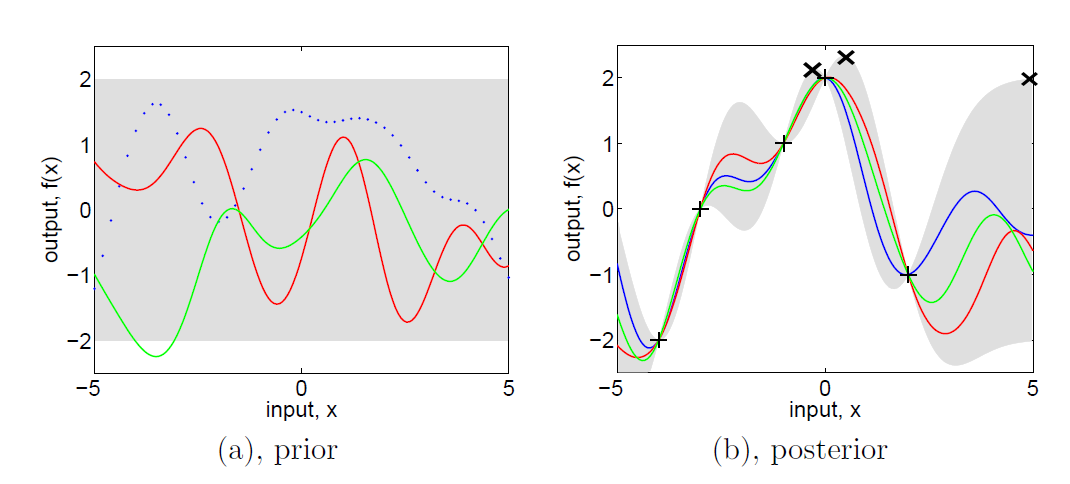
\includegraphics[width=1\linewidth]{bilder/ucb}
	\caption[Gaußprozess im Ausgangszustand (a) und nach dem Lernen von fünf Datenpunkten (b).]{Gaußprozess im Ausgangszustand (a) und nach dem Lernen von fünf Datenpunkten (b). Die drei nächsten Punkte, die per UCB ausgewählt werden sind mit "x" markiert (aus \cite{Rasmussen.2008})}
	\label{fig:ucb}
\end{figure}

Eine Möglichkeit mit dem Dilemma zwischen Exploration und Exploitation umzugehen ist das in \cite{Auer.2002} beschriebene Upper-Confidence-Bound Verfahren. Dabei werden Exploration-Exploitation Probleme als statistischen Prozesse bestehend aus Mittelwert und Varianz aufgefasst.
Der Mittelwert an einem Punkt spiegelt dabei den erwarteten Nutzen wider, eine dem Mittelwert folgende Auswahl bevorzugt also Exploitation von Bereichen, in denen der erwartete Nutzen hoch ist.
Die Varianz spiegelt die Unsicherheit an einem Punkt wider, eine Auswahl nach Varianz bevorzugt die Exploration von Bereichen in denen eine hohe Varianz auftritt, also eben solche Bereiche in denen noch keine Datenpunkte existieren.
Upper-Confidence-Bound kombiniert Mittelwert und Varianz zur Bestimmung der besten Punkte und erreicht damit eine Balance in der sowohl Exploration als auch Exploitation stattfindet.

Gaußprozesse eignen sich durch ihre Eigenschaft an jedem Punkt Mittelwert und Varianz des Gaußprozesses zu berechnen hervorragend zur Anwendung von Upper Confidence Bound.
In \cref{fig:ucb} sind in die in \cref{sub:gp} vorgestellte Abbildung, die drei nächsten Punkte die durch Upper Confidence Bound zu Auswertung bestimmt würden dargestellt.
Die beiden Punkte nahe null stellen dabei Beispiele von Exploitation dar. 
Beide Punkte liegen nahe an einer tatsächlichen Auswertung, durch den hohen Mittelwert in diesem Bereich sollte dieser aber genauer untersucht werden.
Der Punkt am rechten Rand bei $x=5$ stellt ein Beispiel von Exploration dar.
Der Gaußprozess weiß über diesen Bereich noch nichts, folglich besteht dort eine hohe Varianz.
Durch die große Varianz wird dieser Punkt trotz des niedrigen Mittelwerts ausgewählt.

\subsubsection{SAIL}

\begin{algorithm}
	\caption{MAP-Elites} \label{alg:sail}
	\begin{algorithmic}[1]
		\Procedure{MapElites}{$evaluate,categorizationFunction,hyperparameters$}
			\While{$numberEvaluatedSamples < totalSamples$}
				\If{$notInitialized$}
\State $evaluatedSamples \gets evaluate(randomSampling())$ \Comment Evaluate is the real costly Fitness-Function.
\Else
\State $surrogate \gets trainSurrogate(evaluatedSamples)$
\State $acquisitionMap \gets MapElites(acquisitionFunction,categorizationFunction,hyperparameters)$
\State $nextSamples \gets sampleRandomFromMap(acquisitionMap)$ \Comment SAIL utilizes Sobol-sequences to achieve optimal spread of the Sampling
\State $evaluatedSamples \gets evaluatedSamples \cup evaluate(nextSamples)$
\EndIf
			\EndWhile
		\EndProcedure
	\end{algorithmic}
\end{algorithm}

\begin{figure}[h]
	\centering
	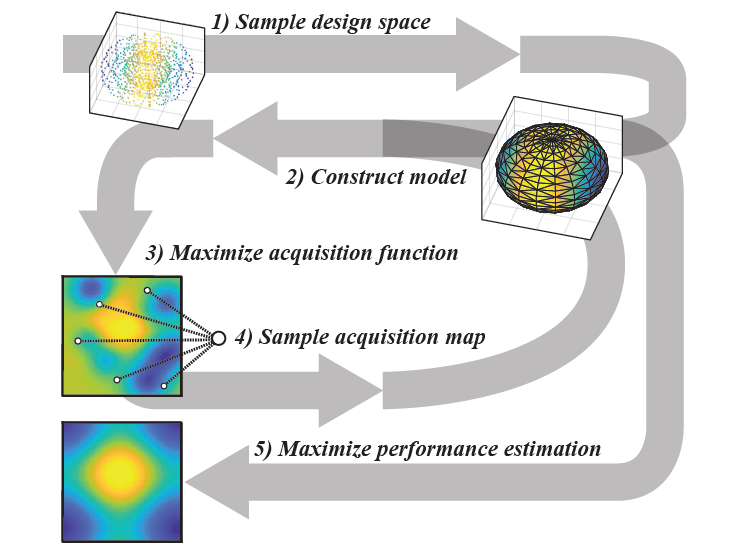
\includegraphics[width=.7\linewidth]{bilder/sail}
	\caption[Teilschritte von SAIL]{Teilschritte von SAIL, 
		1) zufälliges Sampling des Problemraums, 
		2) Trainieren eines Surrogatmodells, 
		3) Erstellung der Akquisekarte mit MAP-Elites mit Upper-Confidence-Bound als Fitness, 
		4) Auswahl der Individuen mit höchstem UCB-Wert und reale Auswertung,
		5) Finale Auswertung mit MAP-Elites
	}
	\label{fig:sail}
\end{figure}

SAIL (Surrogate-Assisted Illumination) ist ein in \cite{Gaier.6152018} beschriebenes Verfahren, welches die in \cref{sub:mapElites} und \cref{sub:surrogate} beschriebenen Ansätze vereint, mit dem Ziel MAP-Elites in rechenintensiven Domänen anwendbar zu machen.

Zur Initialisierung SAILs werden zuerst zufällig Samples ausgewählt und evaluiert.
Um eine gleichmäßige Verteilung der Samples über den Problemraum zu garantieren werden diese Samples nicht aus einer Gleichverteilung, sondern aus einer Sobol Sequenz (\cite{Sobol.1967}) ausgewählt.
Der eigentliche Kern von SAIL ist die graduelle Verfeinerung des Surrogatmodells.
In jeder Iteration der Verfeinerungsschleife wird ein Gaußprozess auf Basis aller bisher ausgewerteten Samples trainiert.
Mit diesem Gaußprozess wird MAP-Elites durchgeführt, wobei als Fitnessfunktion für die Durchführung von MAP-Elites die Akquisefunktion genutzt wird.
Die Akquisefunktion ist dabei Upper Confidence Bound.
Dadurch wird die sogenannte Akquisekarte erzeugt, welche diverse Lösungen enthält, die die Akquisefunktion maximieren.
Aus dieser Akquisekarte werden dann mehrere Lösungen für reale Fitnessevaluationen ausgewählt.
Durch die Nutzung von Upper-Confidence-Bound als Akquisefunktion stellen diese Lösungen Optima bezüglich Exploration und Exploitation dar.
Die ausgewählten Samples werden daraufhin ausgewertet  und den bereits ausgewerteten hinzugefügt, um den Gaußprozess in der nächsten Iteration besser zu trainieren.
Dies kann abhängig von den verfügbaren Rechenkapazitäten beliebig oft wiederholt werden.
Am Ende produziert diese Schleife eine Menge an echten ausgewerteten Samples auf deren Basis der Gaußprozess trainiert werden kann.

In der finalen Auswertung wird dann ein Gaußprozess auf Basis aller ausgewerteten Samples trainiert.
Mit diesem Gaußprozess wird dann ein letztes Mal MAP-Elites durchgeführt, statt der Akquisefunktion wird allerdings die Fitnessfunktion optimiert, die durch den Mittelwert des Gaußprozesses beschrieben wird.
Der Mittelwert des Gaußprozesses an einem Punkt entspricht gerade der mittleren Vorhersage zur Fitness einer realen Auswertung an diesem Punkt.
Damit wird dann eine diverse Vorhersagekarte erzeugt, die die Optima des Gaußprozesses zeigt.
Bei korrekter Parametrisierung von SAIL, dem Gaußprozess, und einer ausreichen großen Anzahl an realen Auswertungen korrespondieren Optima im Gaußprozess mit Optima in der realen Fitnessfunktion.

In \cite{Gaier.6152018} wurde gezeigt, dass dieser Ansatz erfolgreich auf zweidimensionale und dreidimensionale aerodynamische Domänen angewandt werden kann.
Dort wurden per Freiform-Deformation dreidimensionale Objekte deformiert.


\subsection{Constraints in Optimierungsprozessen}
Constraints sind eine Möglichkeit anderweitige Beschränkungen, welche eingehalten werden sollen oder müssen, in einen Optimierungsprozess einzuarbeiten, ohne auf multivariate Optimierung zurückgreifen zu müssen.
Dass Beschränkungen, wie Lösungen aussehen dürfen, existieren ist sehr häufig der Fall.
Die einfachste Möglichkeit ist es die Genotypenkodierung und die Mapping-Funktion so zu wählen, dass nur Lösungen generiert werden können, die die Beschränkung erfüllen.
Ist dies nicht möglich, muss eine explizite Behandlung des Constraints stattfinden.
Constraints lassen sich grundsätzlich in Soft Constraints, bei denen die Nichteinhaltung des Constraints zur Addition von Strafwerten auf die Fitnessfunktion führt, und Hard Constraints, die eine binäre erfüllt/nicht erfüllt Auswahl treffen, unterscheiden.
Welche der drei Arten genutzt wird, hängt stark von der Problemstellung ab.

Auch stellt die Formulierung von Constraints häufig eine Herausforderung dar.
So müssen diese offensichtlich berechenbar sein, Constraints sind allerdings häufig nicht in mathematischer Form formuliert, sondern eher in einer Art die an Requirements erinnert.
Es muss folglich zuerst eine mathematische Formulierung für den Constraint entwickelt werden, die dem Constraint so weit wie möglich entspricht.
Zweitens werden Constraints in einem typischen evolutionären Optimierungsalgorithmus sehr häufig evaluiert werden. 
Das bedeutet, dass die Berechnung des Constraints entweder nicht besonders rechenintensiv sein darf, oder Hilfsmechanismen integriert werden wie beispielsweise die Modellierung des Constraint durch ein Surrogatmodell, wie es in SAIL für die Fitness bereits geschieht.

\subsubsection{Ausschluss durch Definition der Repräsentation}

Die einfachste Art mit äußeren Einschränkungen umzugehen, ist es die Repräsentation des Problems so zu formulieren, dass es nicht möglich ist Phänotypen zu generieren, die den Constraint verletzen.
Im Gegensatz zum Phänotyp, dessen Definition von der Problemdomäne abhängt, kann der Genotyp frei definiert werden.
Die einzigen Kriterien, die der Genotyp erfüllen muss, sind, dass eine Abbildung existiert mit der aus einem Genotyp ein zugehöriger Phänotyp generiert werden kann, dass die Methoden der evolutionären Optimierung, sprich Mutation und Crossover, mit ihm durchgeführt werden, und dass neue zufällige Genotypen generiert werden können.
Die Wahl einer guten Repräsentation des Problems ist einer der wichtigsten Teile der evolutionären Optimierung.
So existieren Beispiele, in denen das gleiche Problem mit einer Repräsentation nicht gelöst werden kann, während dies mit einer anderen Repräsentation möglich ist.
Constraints können in der Wahl der Problemrepräsentation bereits behandelt werden.
Ist es möglich, durch eine kluge Wahl der Repräsentation zu garantieren, dass nur solche Genotypen generiert werden können deren zugehöriger Phänotyp den Constraint erfüllt, ist sichergestellt, dass jede mögliche Lösung valide ist, und der Constraint nicht weiter behandelt werden muss.

Dies hat den Vorteil, dass ungültige Lösungen niemals in den Algorithmus einfließen, und damit weder Rechenkapazitäten für nicht nutzbare Lösungen genutzt werden, noch solche Eigenschaften, durch die eine Lösung die Constraints verletzt, vom Algorithmus überhaupt in Erwägung gezogen werden.
Dies kann eine sehr einfache und effektive Art sein um mit Constraints umzugehen und sollte, sofern es möglich ist, die erste Wahl zu Behandlung von Constraints sein.
Häufig ist es allerdings so, dass die Definition einer Repräsentation, die den Constraint erfüllt, eine große Herausforderung darstellt.
Besonders in solchen Problemdomänen, in denen die Genotyp-Phänotyp Abbildung komplex ist, ist es häufig sehr schwer die Repräsentation so zu wählen, dass sie einen beliebigen Constraint ausschließt.

\subsubsection{Hard Constraints}

Ist es nicht möglich durch die Wahl der Repräsentation Lösungen auszuschließen, die den Constraint verletzen, dann ist ein Hard Constraint die nächste Wahl.
Im Gegensatz zur Wahl der Repräsentation, findet die Auswahl durch einen Hard Constraint auf der Phänotypebene statt.
Dazu existiert eine Funktion die für jeden Phänotyp testet, ob dieser den Constraint erfüllt.
Solche Lösungen, die den Constraint nicht erfüllen werden disqualifiziert, während solche die ihn erfüllen, im Algorithmus genutzt werden dürfen.
Da Constraints immer Constraints des Phänotyps sind, ist die Behandlung dieser auf Phänotypebene einfacher, als der Ausschluss invalider Phänotypen durch Änderung des Genotyps.
Typischerweise werden bei der Nutzung von Hard Constraints an allen Stellen im Algorithmus an denen neue Lösungen generiert werden, sprich Zufallsinitialisierung, Mutation und Crossover, ungültige Lösungen herausgefiltert.

Hard Constraints haben denselben Vorteil wie der Ausschluss durch die Wahl der Repräsentation, ungültige Lösungen niemals in den Algorithmus einfließen, und damit weder Rechenkapazitäten für nicht nutzbare Lösungen genutzt werden, noch solche Eigenschaften, durch die eine Lösung die Constraints verletzt, vom Algorithmus überhaupt in Erwägung gezogen werden.
Im Gegensatz zu dieser Variante muss bei der Nutzung von Hard Constraints, für jedes generierte Individuum getestet werden ob es den Constraint erfüllt.
Dies nimmt Rechenzeit in Anspruch und schränkt die Formulierung der Constraint-Funktion durch die hohe Zahl an Individuen insoweit ein, als dass diese angemessen schnell berechenbar sein muss.



\subsubsection{Soft Constraints}
Soft Constraints disqualifizieren Lösungen, die die Constraints verletzen, nicht.
Stattdessen wird beim Nichterfüllen von Constraints ein Strafwert auf die Kostenfunktion addiert, bzw. von einer Fitnessfunktion subtrahiert.
Dass Lösungen, die die Constraints nicht erfüllen, nicht disqualifiziert werden, hat den Vorteil, dass viele Optimierungsmethoden iterativ zu (lokalen) Optima konvergieren\footnote{Auch ein divergentes Optimierungsverfahren wie MAP-Elites konvergiert zu Optima, es wird nur sichergestellt, das zu einer Vielzahl lokaler Optima konvergiert wird}, 
und diese auch Lösungen, die die Constraints nicht erfüllen, als Trittbretter zu Lösungen, die die Constraints erfüllen, nutzen können.

Soft Constraint eignen sich in Fällen, in denen zu Beginn keine Lösungen bekannt sind, die die Constraints erfüllen, und in denen explorativ nach Lösungen gesucht werden soll, die die Constraints erfüllen.
Auch eignen sie sich für solche Probleme, in denen qualitative Unterschiede bezüglich der Stärke der Verletzung der Constraints zwischen unterschiedlichen Lösungen existieren können.
So kann argumentiert werden, dass im Falle, dass ein Constraint die Einhaltung eines Schwellenwerts ist, eine Lösung, die diesen um 1 überschreitet, qualitativ besser ist als eine, die diesen um 10 überschreitet.

Eine der größten Gefahren bei Soft Constraints ist, dass diese typischerweise als Kostenfunktionen formuliert werden, deren Wert mit der eigentlichen Zielfunktion der Optimierung kombiniert wird.
Eine solche Kombination enthält immer eine Gewichtung für alle Teilfunktionen, aus denen sie besteht.
Diese Gewichtung kontrolliert wie stark die einzelnen Funktionen in die Berechnung der Fitness einfließen.
Oft entsteht die Einführung eines Soft Constraints ein weiteres Problem:
Welche Gewichtung führt zu den besten beziehungsweise gewollten Ergebnissen?
Unter welcher Gewichtung der Algorithmus die qualitativ besten Ergebnisse liefert ist typischerweise nicht klar, bevor dieser mit dieser Gewichtung ausgeführt wird.
Wird eine suboptimale Gewichtung gewählt kann dies dazu führen, dass Constraints über oder unter priorisiert werden, was wiederum zur Folge haben kann, dass entweder Constraints oder das Primärziel ignoriert werden.


\subsubsection{Vergleich}


\begin{table}[h]
	\begin{tabularx}{.9\textwidth}{lXX}\hline
		Variante 		& Vorteile 		& Nachteile \\ \hline
		Repräsentation 	& 
		\begin{itemize}
			\item Behandlung des Constraints im Algorithmus nicht mehr nötig
			\item Keine zusätzlichen Berechnungen notwendig
		\end{itemize} &
		\begin{itemize}
			\item Keine Trittbretter
			\item Formulierung einer passenden Repräsentation in komplexen Domänen häufig aufwendig
		\end{itemize} \\
		Hard Constraint &
		\begin{itemize}
			\item Ergebnis kann keine invaliden Lösungen enthalten
			\item Formulierung des Constraints auf Phänotypebene leichter
		\end{itemize} &
		\begin{itemize}
			\item Keine Trittbretter
		\end{itemize} \\
		Soft Constraint &
		\begin{itemize}
			\item Nutzung von Trittbrettern wird ermöglicht
		\end{itemize} &
		\begin{itemize}
			\item Ergebnis kann invalide Lösungen enthalten
		\end{itemize} \\
	\end{tabularx}
	\caption{Vor-/Nachteile der verschiedenen Möglichkeiten einen Constraint zu modellieren}
	\label{tab:methods_constraint}
\end{table}
	


Welcher der drei Ansätze am besten für ein Problem ist, hängt von dessen Formulierung ab.
Grundsätzlich sollte der Ausschluss durch Modellierung Hard Constraints und diese wiederum Soft Constraints vorgezogen werden.
Wenn der Ausschluss durch die Modellierung allerdings mit hohem Aufwand verbunden ist, wie es in komplexen Domänen häufig der Fall ist, sollten stattdessen Hard Constraints in Erwägung gezogen werden.
Wenn die Vermutung besteht, dass zum Erreichen ausreichend guter Lösungen Trittbrettlösungen, die die Constraints nicht erfüllen, benötigt werden sollten stattdessen Soft Constraints genutzt werden.

\clearpage

\section{Methode}

In diesem Kapitel werden die in \cref{sub:grundlagen} besprochenen Techniken auf zwei Domänen angewandt.
Die erste dieser Domänen ist die Generierung von verformten Radkästen eines Velomobils, unter Beachtung eines Constraints.
Die zweite Domäne ist die explorative Untersuchung verschiedener Bauteilformen an der Unterseite eines E-Rollers.
In beiden Domänen ist die Verformung dreidimensionaler Bauteile und die darauffolgende Bewertung des Effektes auf die Aerodynamik, den diese Verformung hat, Untersuchungsziel.
Auf die domänenübergreifende Teile der Repräsentation wird in \cref{sub:representation} eingegangen.
Darauffolgend wird in \cref{sub:method_wheelcase} \cref{sub:method_escooter} auf die Spezifika, wie Constraints und Featurewahl, der Radkasten- beziehungsweise E-Roller-Domäne eingegangen.

\subsection{Repräsentation der Domänen}
\label{sub:representation}

In beiden Domänen geht es um die Deformation von dreidimensionalen Bauteilen und die Bewertung der aerodynamischen Effekte solcher Deformationen.
D.~h. es wird eine robuste Methode benötigt, um dreidimensionale Bauteile zu deformieren und solche Deformationen auf wenige Parameter reduzieren zu können.
Eine Methode, die diese Rahmenbedingungen erfüllt ist die Freiformdeformation \cite{Sederberg.1986} auf die in \cref{sub:ffd} genauer eingegangen wird, die Deformationen von komplexen geometrischen Objekten anhand Verschiebungen von Rahmenpunkten ausdrücken kann.
Für aerodynamische Simulationen wird in beiden Domänen OpenFoam verwendet, ein Open-Source-Programm welches unter anderem fähig ist Windkanalsimulationen durchzuführen.
Auf die genaueren Eigenschaften von OpenFoam und den Aufbau einer passenden Simulationsumgebung wird in \cref{sub:openfoam} eingegangen.

\subsubsection{Freiformdeformation}
\label{sub:ffd}
\begin{figure}[h]
	\centering
	\begin{minipage}{0.45\textwidth}
		\centering
		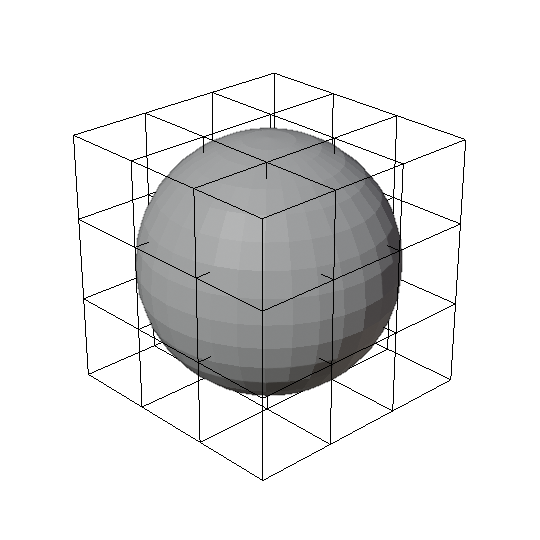
\includegraphics[width=1\linewidth]{bilder/sphere_lattice}
		\caption{3D-Mesh einer Kugel in 4x4x4 FFD-Box}
		\label{fig:ffd_undeformed}
	\end{minipage}\hfill
	\begin{minipage}{0.45\textwidth}
		\centering
		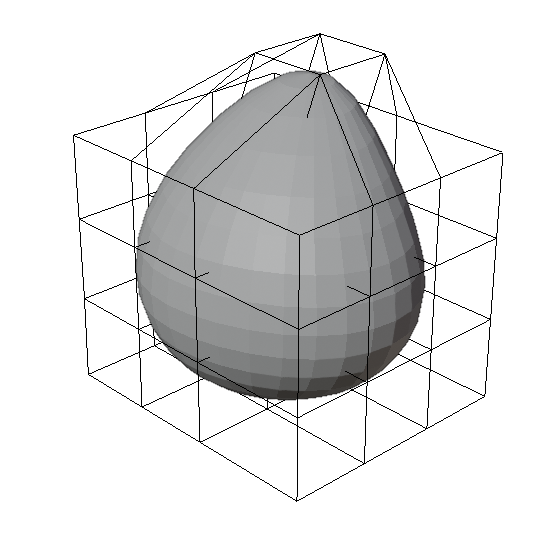
\includegraphics[width=1\linewidth]{bilder/sphere_lattice_deformed2}
		\caption{Deformiertes 3D-Mesh erzeugt durch Bewegung der Deformationspunkte}
		\label{fig:ffd_deformed}
	\end{minipage}
\end{figure}
Freiformdeformation ist ein in \cite{Sederberg.1986} beschriebenes Verfahren zu Deformation von geometrischen Objekten.
Mithilfe der Freiformdeformation können beliebige dreidimensionale Meshes robust deformiert werden.
Dazu wird eine Box aus Kontrollpunkten erzeugt, die manipuliert werden können, um das Mesh zu deformieren.
In \cref{fig:ffd_deformed} ist das 3D-Mesh einer Kugel umgeben von einer FFD-Box aus vier Punkten in jeder Dimension.
Damit ergeben sich 64 Deformationspunkte.
Jeder dieser Kontrollpunkte kann dann anhand von Verformungsparametern verschoben werden, wodurch für alle Punkte innerhalb der FFD-Box eine Verschiebung berechnet wird, die von der relativen Position des Punktes zum Kontrollpunkt abhängt.
Eine deformierte Variante der Kugel ist in \cref{fig:ffd_deformed} abgebildet.
Dort wurden alle Punkte der rechten Ebene der FFD-Box nach außen bewegt und die vier inneren Punkte auf der Oberseite der FFD-Box nach oben und hinten bewegt.
Die Knoten der Kugel werden durch die Freiformdeformation entsprechend bewegt, wodurch das deformiert Mesh entsteht.
So können beliebige dreidimensionale Meshes robust anhand einiger Punkte deformiert werden.
Auch können Deformationen durch relativ wenige Deformationsparameter definiert werden.
Im Beispiel läge die Anzahl an Freiheitsgraden bei $64 * 3 = 192$.
Durch eine weitere Auswahl an welchen Punkten Deformationen in welche Richtungen 
\footnote{Deformation in x, y, z finden jeweils separat statt}
stattfinden dürfen, kann diese Zahl noch weiter reduziert werden.
Dadurch eignet sich das Verfahren zur Anwendung in evolutionären Algorithmen, in denen die Anzahl der möglichen Freiheitsgrade, was der Länge des Genoms entspricht, nach oben weich begrenzt ist.
Dadurch das nur die Punkte des Meshes ihre Position ändern, hat das Verfahren, den Vorteil das die Dreiecke erhalten bleiben und somit beispielsweise das Entstehen von Löchern bei korrekter Anwendung praktisch ausgeschlossen ist.

\subsubsection{OpenFOAM}
\label{sub:openfoam}
OpenFoam \cite{OpenCFD.} ist eine Open-Source-Programm zur Durchführung von Fluiddynamiksimulationen.
Berechnungen in OpenFOAM sind in sogenannten "Cases" organisiert auf die nacheinander OpenFoam-Funktionen angewandt werden.
Diese Cases bestehen aus einer Basisstruktur, die Initiale Startparameter, sowie Dateien zur Steuerung von OpenFoam enthalten.
%Diese basis ist in den Ordnern \textit{domains/wheelcase/pe} und \textit{domains/escooter/pe} zu finden.
Diese Basis enthält typischerweise Skripts um die gesamte Kette aus verschiedenen OpenFoam Funktionen, die zur Durchführung einer Simulation notwendig sind, auszuführen, sowie ein Skript, welches den Case wieder in den Startzustand versetzt.
Außerdem enthält diese Basis das Verzeichnis system, das C++-Dictionaries enthält, mit denen die einzelnen OpenFoam Funktionen parametrisiert und gesteuert werden.
Für jede der genutzte OpenFoam Funktion existiert dort eine Datei, in der beschrieben wird was die entsprechende Funktion wie tun soll. 
Zuletzt befindet sich in diesem Ordner auch noch der Initiale Startzustand, mit dem die Simulation beginnt.

OpenFoam bietet native Unterstützung von Parallelität über MPI \cite{OpenMPI.}.
Neben den Funktionen um die korrekte Aufteilung eines Cases auf mehrere Prozessoren aufzuteilen und am Ende wieder zu rekonstruieren sind zwei Funktionen und deren dazugehörige Dateien hervorzuheben.

Diese beiden wichtigsten genutzten OpenFoam-Funktionen sind snappyHexMesh und simpleFoam.
Mit snappyHexMesh, dessen Parametrisierung in \path{snappyHexMeshDict} zu finden ist, wird aus dem STL das für die Fluiddynamiksimulation benötigte Mesh generiert. Über snappyHexMesh kann die Auflösung des in der Fluiddynamiksimulation genutzten Meshes kontrolliert werden.
Die Parametrisierung von snappyHexMesh ist deshalb besonders wichtig, da die Auflösung des Meshes die Simulation maßgeblich beeinflusst.
SnappyHexMesh ist ein auf Octrees (\cite{Meagher.1982}) basierender Verfeinerungsalgorithmus.
Die Parametrisierung von snappyHexMesh kontrolliert welche Bereiche stärker verfeinert werden.
In diesen Bereichen wird der Baum tiefer und es werden mehr Zellen generiert.
In der darauffolgenden Simulation bilden Zellen die atomare Einheit, wenn in bestimmten Bereichen nicht weit genug verfeinert wurde, besteht in der Simulation überhaupt nicht die Möglichkeit der Realität entsprechende Messwerte in dieser Zelle zu berechnen.
Mit wachsender Anzahl der Zellen wächst allerdings auch die Zeit die für Verfeinerung und Simulation benötigt wird.
Die korrekte Auswahl in welchen Bereichen es nötig ist für eine korrekte Simulation stärker zu verfeinern und in welchen Bereichen eine weitere Verfeinerung nur weitere Berechnungskomplexität ohne Informationsgewinn hinzufügt. 

Die zweite dieser Funktionen ist die eigentliche Fluiddynamiksimulation.
Abhängig von den benötigten Simulationsparametern stellt OpenFoam einige unterschiedliche Solver bereit.
Da die Strömungsgeschwindigkeiten der Simulation weit unter $0.3Ma$ bleiben kann die Strömung als inkompressibel behandelt werden (\cite{Anderson.2017}).
Es existieren mehrere OpenFoam Solver für inkompressible Strömungen aus denen simpleFoam ausgewählt wurde.
simpleFoam implementiert den SIMPLE (Semi-Implicit Method for Pressure Linked Equations) Algorithmus, der in \cite{Caretto.1973} beschrieben wurde.
Für die hier benötigten Werte reicht simpleFoam vollkommen aus.
\todo{eingehen auf simple foam}
Zudem werden die Koeffizienten der auf das Objekt wirkenden Kräfte berechnet, welche für die Berechnung der Fitness benötigt werden. 

\subsubsection{Parametrisierung des Gaußprozesses}

Die Parametrisierung des Gaußprozesses besteht aus drei Schritten.
Zuerst werden die Funktionen für Kovarianz, Mittelwert und Wahrscheinlichkeit ausgewählt werden.
Daraufhin müssen die Hyperparameter dieser drei Funktionen gesetzt werden.
Da das Setzen der richtigen Hyperparameter schwer ist, können diese daraufhin, nachdem Datenpunkte vorhanden sind, so optimiert werden, dass die Daten am besten beschrieben werden.

Die erste Funktion, die ausgewählt wurde, ist die Kovarianzfunktion.
Es wurde die isotropische Squared exponential Konvarianz Funktion 
\[
	k(x,x') = \sigma_f * \exp\left(-\frac{(x-x')^2}{2\ell^2}\right)
\]
gewählt.
Diese besitzt die Hyperparameter $\sigma_f$, welcher die Standardabweichung des Signals bestimmt, und $\ell$, wodurch das Längenmaß bestimmt wird.
Die Squared exponential Funktion wird manchmal auch als Radial basis function (RBF) bezeichnet und stellt einen der meist genutzten Kernelfunktionen dar.
Da sie unendlich differenzierbar ist, werden sehr glatte Funktionen generiert.
\todo{universal kernels}
Das ist von Vorteil
Isotropisch bedeutet in diesem Fall, dass das Längenmaß $\ell$ in allen Dimensionen gleich ist.
Da alle Dimensionen auf das Intervall $[0;1]$ normiert sind, kann das gleiche Längenmaß für alle Dimensionen genutzt werden.
Die Nutzung eines Längenmaßes vereinfacht die Parametrisierung, häufig kann es trotzdem der Fall sein, dass bestimmte Dimensionen wichtiger für die Korrelation zwischen zwei Punkten sind, eine Möglichkeit damit umzugehen ist das sogenannte Automatic relevance determination (ARD), wodurch jede Dimension ein unabhängiges Längenmaß erhält.

Die zweite Funktion die ausgewählt werden muss ist die Mittelwertsfunktion. Da unser Wissen über den Problemraum sich hauptsächlich auf Hypothese und Schätzungen beschränkt wurde hier die einfachste der Mittelwertsfunktionen gewählt. 
Der konstante Mittelwert
\[
	m(x) = c
\]
besitzt nur einen Hyperparameter $c$, der festlegt auf welcher Konstanten der Mittelwert liegt.

Als letztes muss noch eine Entscheidung bezüglich der Wahrscheinlichkeitsfunktion getroffen werden.
Diese steuert die Varianz des Gaußprozesses.
Da es keinen Grund gibt davon auszugehen, dass diese nicht Normalverteilt ist, wurde hier die Normalverteilung mit
\[
	\mathcal{N}(y_i \mid f_i, \sigma_n^2) = \frac{1}{\sqrt{2\pi*\sigma_n^2}}*\exp\left(-\frac{(y_i - f_i)^2}{2\sigma_n^2}\right)
\]
gewählt.
Auch diese Funktion hat nur einen Hyperparameter $\sigma_n$, der steuert wie breit das Varianzband ist.
Bei einem stärkeren Rauschen der Daten wird ein größeres $\sigma_n$ benötigt um nahe Datenpunkte mit sehr verschiedenen Werten beschreiben zu können.

Die initiale Parametrisierung der Hyperparameter erfolgte gemäß 

\begin{table}[h]
	\centering
	\begin{tabularx}{.25\textwidth}{ll}\hline
		$\ell$ & $0.5$ \\
		$\sigma_f$ & $0$ \\
		$c$ & $0$ \\
		$\sigma_n$ & $1$ \\
	\end{tabularx}
	\caption{Initiale Hyperparameter des Gaußprozesses}
	\label{tab:initialParams}
\end{table}


\subsection{Radkästen des Velomobils}
\label{sub:method_wheelcase}
\begin{figure}[h]
	\centering
	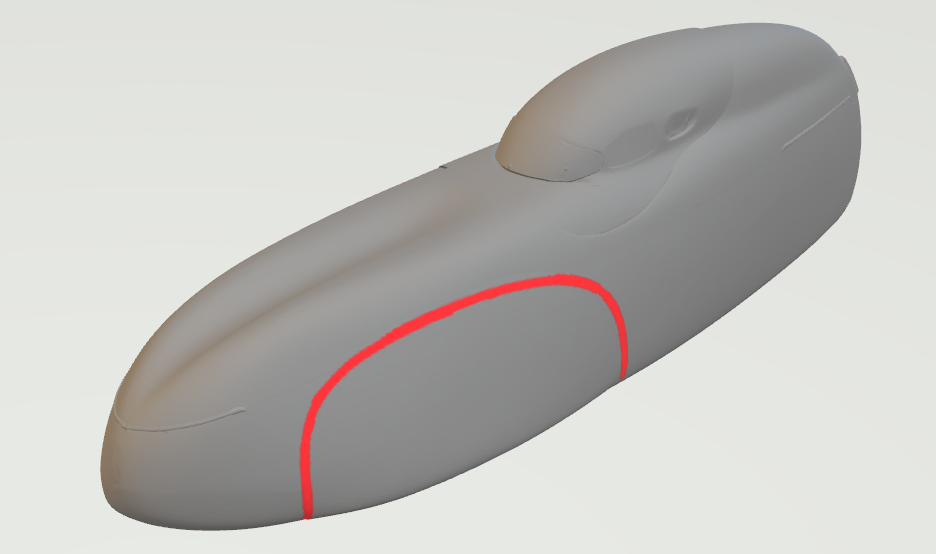
\includegraphics[width=.8\linewidth]{bilder/velo_wheelcase}
	\caption{Radkasten des Velomobils}
	\label{fig:wheelcase}
\end{figure}

Die erste Problemdomäne stellt die Optimierung der Radkästen eines Velomobils dar.
Da die momentanen Radkästen den Lenkausschlag des Velomobils erheblich einschränken, besteht das Ziel hierbei Radkästen zu generieren, die den maximalen, oder zumindest einen weiteren Lenkausschlag als den momentan möglichen, ermöglichen und dabei trotzdem gute aerodynamische Eigenschaften aufweisen.
Es ist zu erwarten, dass eine zusätzliche Fokussierung auf ein zweites Ziel, mit einer Qualitätsabnahme des ersten Ziels verbunden ist.
%Trotzdem ergibt die Einführung eines Constraints nur Sinn, wenn die Abnahme an Optimalität bezüglich des Primärziels gering genug ist um eine Zunahme an Optimalität bezüglich des Sekundärziels vertretbar zu machen.
%Ziel der Einführung eines Constraints ist es einen maximalen Effekt bezüglich dessen Erfüllung durch eine minimalen Optimalitätsabnahme der Zielfunktion zu erreichen. 
Das Ziel besteht also darin Lösungen zu entwickelt, welche durch minimalen Fitnessverlust einen maximalen Constraintgewinn möglich machen.

Da das Velomobil symmetrisch gebaut ist, wurde angenommen, dass die Verformungen des linken und rechten Radkastens symmetrisch sind.
Im Folgenden wird bei allen Beschreibungen von Deformationen vom rechten Radkasten ausgegangen.
Die Deformationspunkte zur Deformation des linken Radkastens ergeben sich durch eine Invertierung der y-Koordinate.
Außerdem finden alle Deformationen in y-Richtung für den linken Radkasten negativ statt.
Dies führt dazu, dass der linke Radkasten symmetrisch zum rechten verformt wird.
Dadurch kann die Anzahl an benötigten Freiheitsgrade halbiert werden. 
Auch die Berechnungen des Constraints und der Kategorisierung können dadurch nur für den rechten Radkasten durchgeführt werden, was auch dafür den benötigten Aufwand halbiert.

Um möglichst glatte Übergänge zwischen Radkasten und Velomobil herstellen zu können wurden die Radkästen nicht separat verformt un daraufhin mit dem Rest des Velomobils kombiniert, sondern es wurden mit FFD-Boxen um die Radkästen das komplette Modell verformt.
Dies ist zwar eine leichte Abweichung von der Aufgabenstellung, allerdings sind scharfe Ränder aerodynamisch suboptimal und daher zu vermeiden, und genau das wird dadurch erreicht.

\subsubsection{OpenFOAM}

Es wird wie bereits in \cref{sub:openfoam} beschrieben snappyHexMesh zur Konstruktion der Volumenmeshes genutzt.
Zur Verfeinerung wurde der "distance" Modus genutzt, bei dem Zellen abhängig von ihrer Distanz zu einer Oberfläche stärker verfeinert werden.
Die Oberfläche zur Messung dieser Distanz ist in diesem Fall das Velomobil.
Somit kann erreicht werden, dass Zellen nahe des Velomobils stark verfeinert werden, und weiter entfernte Zellen nicht zu stark verfeinert werden.
Da aerodynamische Effekte primär am Velomobil stattfinden bot diese Einstellung eine Möglichkeit dafür angemessene Verfeinerungen herzustellen.
Als Parametrisierung wurde (0.2 5) (0.5 4) (1.0 2) gewählt, d.h. alles mit einer Entfernung kleiner $0.2m$ zum Velomobil wird zu Level 5 verfeinert, alles mit einem Abstand bis $0.5m$ mit Level 4 und alles mit einem Abstand bis zu $1m$ mit Level 2.

\begin{figure}[h]
	\centering
	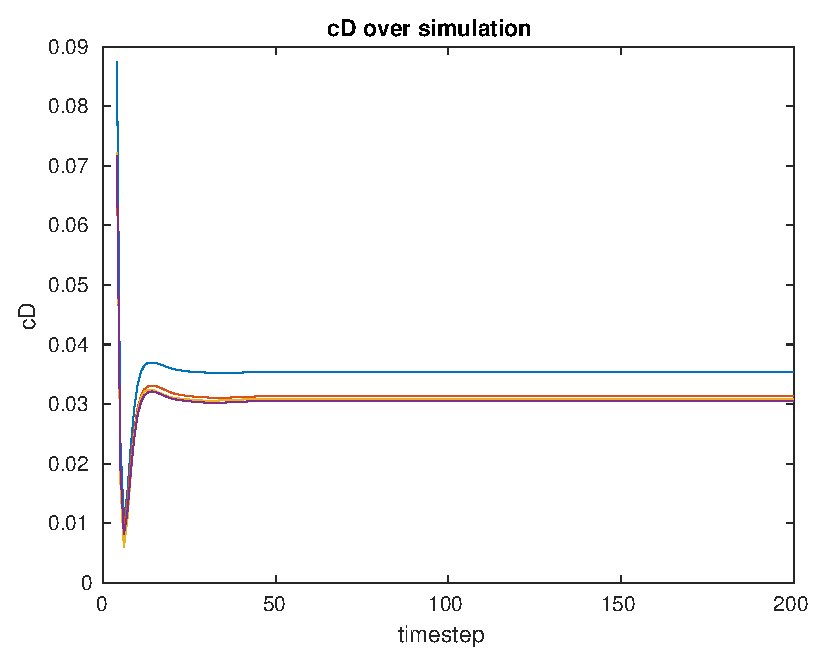
\includegraphics[width=.8\linewidth]{bilder/wheelcaseCDConvergence}
	\caption{Luftwiderstandswerte über Simulationen von vier zufällig verformten Radkästen}
	\label{fig:wheelcase_convergence}
\end{figure}
Es wurden mehrere OpenFoam-Simulationen des Velomobils durchgeführt um zu testen, ob und wann die berechneten cD-Werte ausreichend konvergieren.
In \cref{fig:wheelcase_convergence} sind die berechneten cD-Werte über den Simulationslauf dargestellt. 
Es ist erkennbar, dass diese zum Start der Simulation stark schwanken, sich aber relativ schnell auf den finalen Wert einpendeln.
Ungefähr zwischen 50 und 100 Sekunden sind die cD-Werte ausreichen konvergiert.
Da die Konvergenz für unterschiedliche Formen unterschiedlich erfolgt wurden die cD-Werte von Sekunden bis Sekunden gemittelt, um die Fitness zu berechnen.
Offensichtlich reichen 200 simulierte Sekunden aber aus, um aussagekräftige Ergebnisse zu erlangen.



\subsubsection{Constraint}
%\begin{figure}[h]
%	\includegraphics[width=.5\linewidth]{}
%	\includegraphics[width=.5\linewidth]{}
%	\caption{}
%	\label{fig:steering_volume}
%\end{figure}
\begin{figure}[h]
	\centering
	\begin{minipage}{0.45\textwidth}
		\centering
		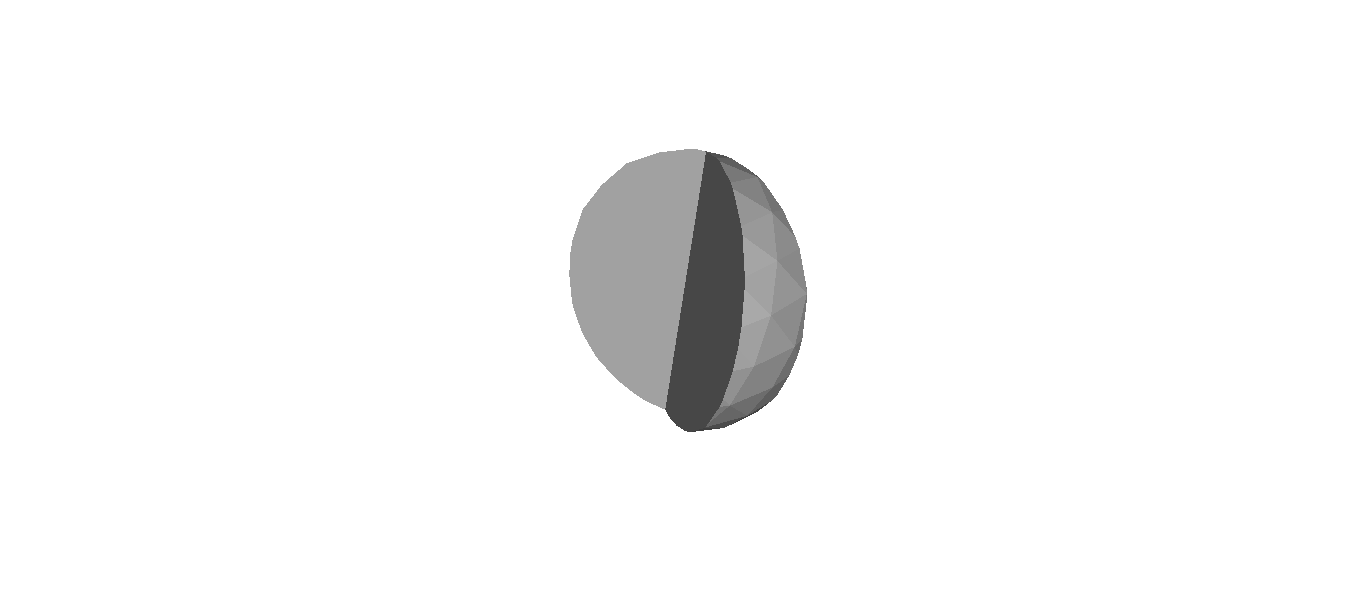
\includegraphics[width=1\linewidth]{bilder/radausschlag.png}
		\caption{Das modellierte Radausschlagsvolumen $FV_{radausschlag}$}
		\label{fig:steering_volume}
	\end{minipage}\hfill
	\begin{minipage}{0.45\textwidth}
		\centering
		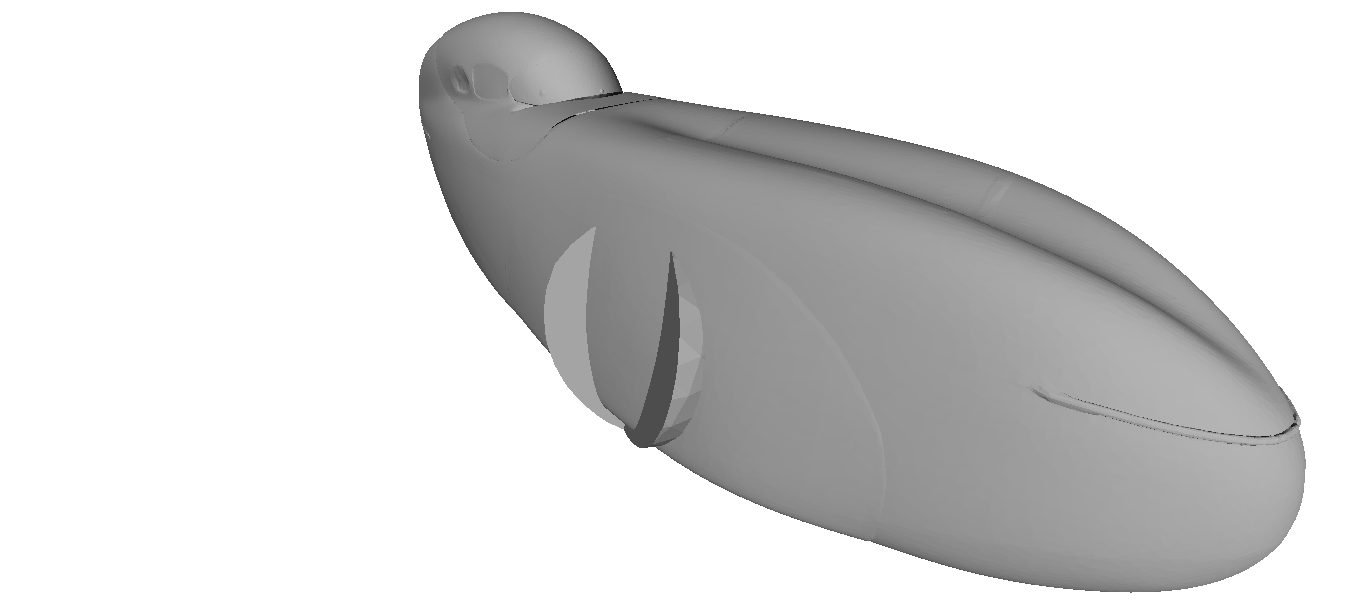
\includegraphics[width=1\linewidth]{bilder/radausschlag_inclVelo.png}
		\caption{Radausschlagsvolumen $FV_{radausschlag}$ mit Velomobil}
		\label{fig:steering_volume_with_velo}
	\end{minipage}
\end{figure}
Zur Erfüllung des Constraints wurden alle möglichen Radausschläge als Mesh modelliert.
Dafür wurden aus einer Kugel entsprechend des maximalen Radausschlags nach rechts und links ein dreieckiges Stück ausgeschnitten.
Zusätzlich wurde die innere Hälfte der Kugel entfernt, da dort keine Überschneidungen stattfinden, und durch deren Entfernen, Berechnungen effizienter sind.
Das Mesh $FV_{radausschlag}$ ist in Abb. \cref{fig:steering_volume} alleine, in Abb. \cref{fig:steering_volume_with_velo} zusammen mit dem restlichen Velomobil dargestellt.
Es ist klar zu Erkennen, dass dieses Volumen die unverformten Radkästen schneidet und diese den maximalen Lenkausschlag nicht ermöglichen.
 

\begin{table}[h]
	\begin{tabularx}{.5\textwidth}{ll}\hline
		
		Position & \\
		\hline
		x &	$926mm$ \\
		y &	$343mm$ \\
		z &	$205mm$	\\
	\end{tabularx}
	\begin{tabularx}{.5\textwidth}{ll}\hline
		Rotation & \\ \hline
		$\phi$ & $16,6\degree$ \\
		$\theta$ & $0\degree$ \\
		$\psi$ & $0\degree$ \\
	\end{tabularx}
	\begin{tabularx}{.5\linewidth}{ll}
		Radius des Rads & $230mm$ \\
		Radausschlag & $\pm24,37\degree$\\
		
	\end{tabularx}

\label{tab:wheel_params}
\caption{Parameter Radausschlag. Ursprung des Koordinatensystems für Position auf Boden an der Spitze des Velomobils. Linkshändiges Koordinatensystem mit z Höhenachse und Velomobil in -x-Richtung ausgerichtet.}
\end{table}

%\begin{figure}[h]
%	\centering
%	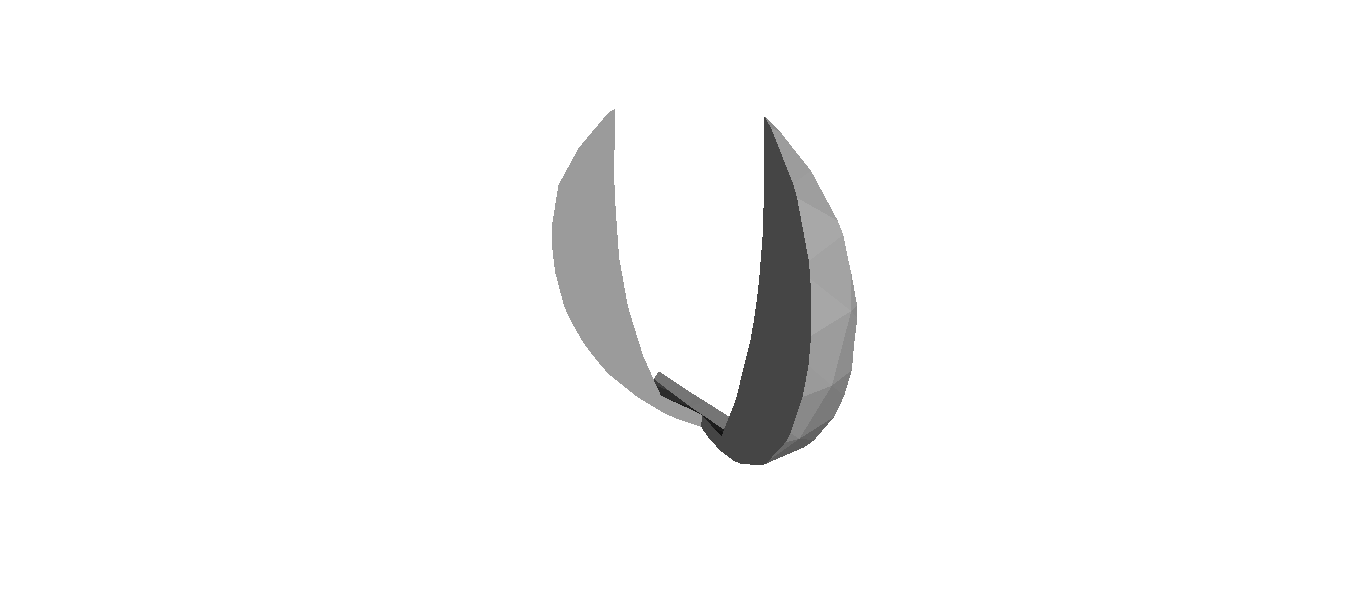
\includegraphics[width=.5\linewidth]{bilder/difference.png}
%	\caption{Das Differenzvolumen für den unverformten Radkasten. Aus diesem wird der Strafwert berechnet}
%	\label{fig:diff_volume}
%\end{figure}
\begin{figure}[h]
	\centering
	\begin{minipage}{0.45\textwidth}
		\centering
		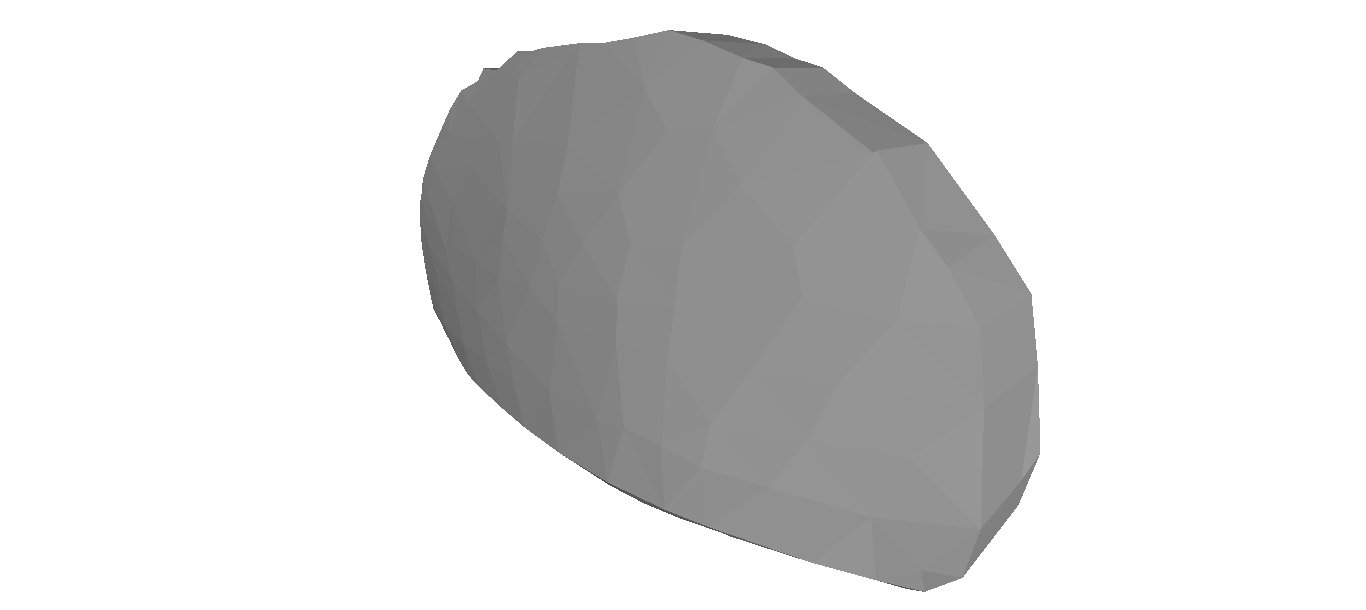
\includegraphics[width=.5\linewidth]{bilder/simplified_wheelcase}
		\caption{Das vereinfachte, geschlossene Mesh des Radkastens $FV_{radkasten}$}
		\label{fig:wheelcase_volume}
	\end{minipage}\hfill
	\begin{minipage}{0.45\textwidth}
		\centering
		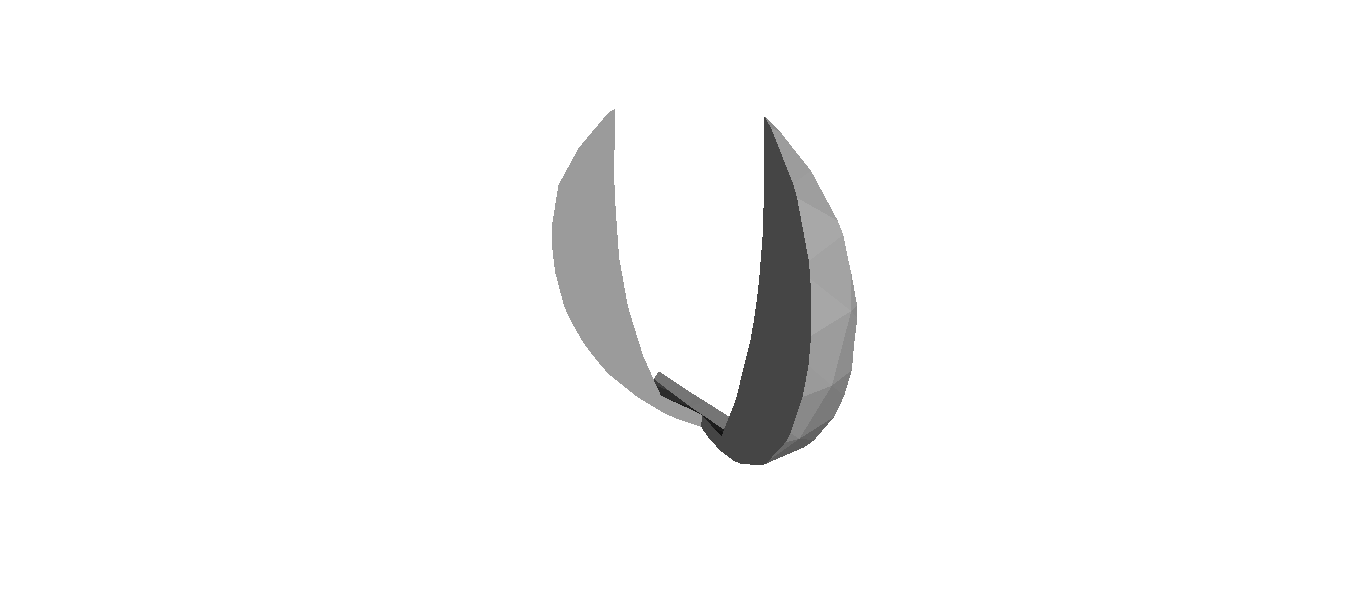
\includegraphics[width=.5\linewidth]{bilder/difference.png}
		\caption{Das Differenzvolumen $FV_{diff}$ für den unverformten Radkasten. Aus diesem wird der Strafwert berechnet}
		\label{fig:diff_volume}
	\end{minipage}
\end{figure}
Da ein Ziel darin bestand, den Constraint nicht als binäres, erfüllt/nicht erfüllt Problem zu definieren, da zwischen zwei Lösungen, die den Constraint nicht erfüllen trotzdem qualitative Unterschiede bestehen können wie stark der Constraint verletzt wird, wird ein Soft Constraint zur Modellierung gewählt.
Dazu wird die Meshdifferenz des Radausschlags und des verformten Radkastens berechnet um $FV_{diff} = FV_{radausschlag} - FV_{radkasten}$ zu ermitteln.
Das Ergebnis einer solchen Meshdifferenz für den unverformten Radkasten ist in \cref{fig:diff_volume} abgebildet.
Die Größe des Volumens $V(FV_{diff})$ wird zur Berechnung des Constraints herangezogen.
Zwar besteht keine direkte Kausalität zwischen diesem Volumen und dem maximalen möglichen Radausschlag aber die Vermutung, dass ein geringeres Volumen dieser Differenz mit größerem möglichen Radausschlag korreliert ist, liegt nahe.
%als Constraint das Differenzvolumen des Radausschlags minus verformten Radkastens gewählt.

Da alle generierten Verformungen der Radkästen symmetrisch sind, wird der Constraint jeweils nur für den rechten Radkasten berechnet.
Zur Berechnung der Differenz zwischen Radausschlagsvolumen und Radkasten wird die Bibliothek \textit{gptoolbox} \cite{gptoolbox.b} genutzt, zur Generierung von Tetraedermeshes zur Volumenberechnung \textit{TetGen} \cite{Si.2015}.
%Ein Beispiel des Differenzvolumens zur Constraintberechnung ist in Abb. \cref{fig:diff_volume} zu sehen.
%Dieses Volumen stellt die Differenz des Radausschlagvolumens und des unverformten Radkastens dar.
Um die Meshdifferenz berechnen zu können wurde der rechte Radkasten zudem geschlossen.
Da die Constraintberechnung in jeder Generation für jedes Kind erfolgen muss wurde der Radkasten außerdem vereinfacht um die Berechnung  des Constraints ausreichend schnell durchführen zu können.
Um den Strafwert $p$ für ein Individuum zu berechnen wird $V(FV_{diff})$ des Individuums berechnet und in Relation zum Außenvolumen des unverformten Radkastens gesetzt \footnote{Für den unverformten Radkasten beträgt das Differenzvolumen ca. $1,6L$}.
Erfüllt ein Individuum den Constraint gleich gut wie der unverformte Radkasten gilt $p=1$.
Ist ein Individuum besser gilt $0\leq p < 1$, ist es schlechter gilt $p>1$.
\[
	p = \frac{V(FV_{diff})}{V(FV_{diffUnverformt})}
\]

Auch wenn die genutzten Bibliotheken zwar recht robust sind ist es trotzdem so, dass sie in ihrer Kombination aber immer noch für ca. 1 aus 10000 Lösungen abstürzen.
Statt den Grund dieser Abstürze zu ermittel, wurde deren Häufigkeit als gering genug eingestuft, als dass dies nicht nötig ist.
Stattdessen werden solche Lösungen im Algorithmus als unendlich schlecht bewertet und damit ausgeschlossen.

Da sich der Constraint durch die Vereinfachung des Radkastens ausreichend schnell berechnen ließ, dass eine direkte Berechnung dessen für jedes Individuum zeitlich möglich war, wurde dies getan.
Das Trainieren eines zweiten Surrogatmodells zur Modellierung des Constraints hätte einen nicht unerheblichen Komplexitätszuwachs bedeutet , der an dieser Stelle nicht nötig war.
Also wurde der Strafwert mit Gewicht $w_{constraint} \geq 0$ gewichtet in die Fitnessfunktion integriert und als $p*w_{constraint}$ auf die Fitness jedes Individuums addiert
\footnote{Die vorliegende SAIL-Implementation minimiert, Addition positiver Werte ist folglich Strafe}.
Allerdings wurde der Strafwert zusätzlich noch in die Akquisefunktion, mit der innerhalb von SAIL die Akquisekarte zur Auswahl neuer Individuen zur Auswertung stattfindet auf die gleiche Weise integriert. Das hat den Grund, dass das Gaußprozessmodell in solchen Bereichen bevorzugt Exploitation durchführen soll, die sowohl bezüglich der Aerodynamik, als auch bezüglich des Constraints eine gewisse Optimalität aufweisen, da genau in diesen Bereichen, in der finalen Auswertung von MAP-Elites solche Lösungen zu erwarten sind, die bezüglich der Kombination dieser beiden Kriterien optimal sind.


\subsubsection{Wahl der Features}
%Die Kategorisierung wird von der \path{wheelcase_Categorize.m} verwaltet.

Als erste Kategorie wurde die Breite des Velomobils gewählt.
Diese Kategorie wurde deshalb gewählt, da hier sehr klare Hypothesen aufgestellt werden können, wie die Breite des Velomobils mit der Aerodynamik und dem Constraint interagiert.
Die erste Hypothese, die aufgestellt werden kann ist, dass breiteren Velomobilen die Erfüllung des Constraints leichter fällt. Es wäre also zu erwarten, dass breitere Velomobile den Constraint tendenziell besser erfüllen, als schmalere.
\begin{itemize}
	\item Breitere Velomobile sind positiv mit Erfüllung des Constraints korreliert.
\end{itemize}
Auch kann die Hypothese aufgestellt werden, dass die Breite negativ mit dem Luftwiderstandsbeiwert korreliert ist.
\begin{itemize}
	\item Breitere Velomobile sind negativ mit Luftwiderstandsbeiwert korreliert.
\end{itemize}
Insgesamt wäre also zu vermuten, dass entlang dieser Achse der Luftwiderstandsbeiwert zunimmt, während der Strafwert des Constraints abnimmt.
%Der Test ob diese Erwartungen erfüllt sind stellt eine einfache Möglichkeit zur semantischen Verfifizierung der Ergebnisse dar.

Als zweite Kategorie wurde die x-Koordinate des breitesten Punkts gewählt.
Da das Velombil in negative x-Richtung ausgerichtet ist, bedeuten kleinere Werte hier, dass der Punkt weiter vorne liegt, größere, dass er weiter hinten liegt.
Zu dieser Kategorie lassen sich keine so direkten Hypothesen aufstellen wie zur ersteren.
Die Frage, ob sich hier klare Tendenzen bezüglich der aerodynamischen Eigenschaften und/oder des Constraints aufzeigen ist auch ein Ziel der Untersuchung.

Da auch die Kategorisierung so häufig stattfindet, wird auch diese mit dem für die Berechnung des Constraints vereinfachten Modell des Radkastens durchgeführt. 
Dies stellt keinen signifikanten Verlust an Genauigkeit in der Kategorisierung dar, da sich die am feinsten gemeshten Teile des Radkastens an dessen Rändern befinden.
Gerade die sind aber die Teile des Radkastens, die am unwahrscheinlichsten den breitesten Punkt darstellen.
Auch führen minimale Genauigkeitsfehler in der Kategorisierung nicht dazu, dass die von MAP-Elites geforderte Lokalität verletzt wird.
Der Geschwindigkeitsgewinn bei der Berechnung hingegen macht es möglich solche Kategorien, für die eine Verformung des Radkastens notwendig ist, zu wählen, was in Relation einen wesentlich größeren Gewinn darstellt.

\subsection{E-Roller}
\label{sub:method_escooter}
\begin{figure}[h]
	\centering
	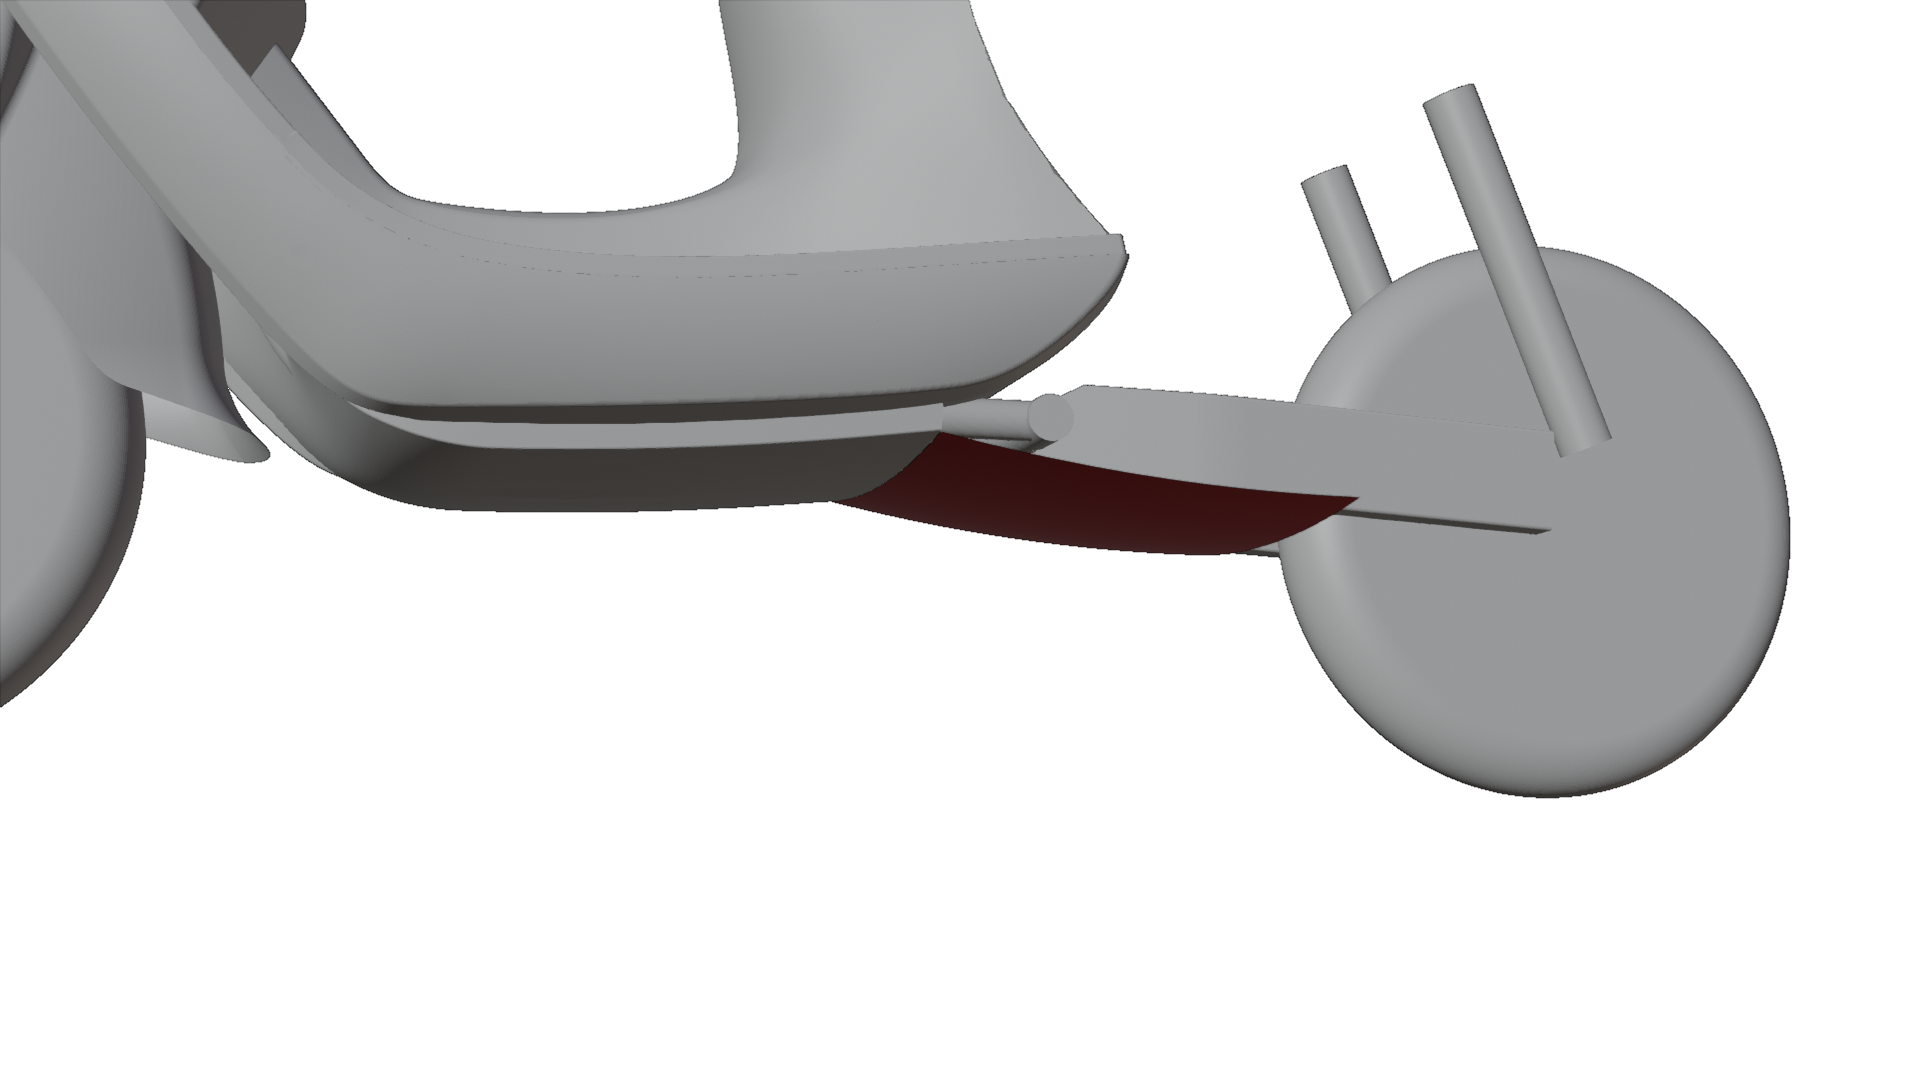
\includegraphics[width=.8\linewidth]{bilder/escooter_component}
	\caption{E-Roller (weiß) und das zu deformierende Bauteil (rot)}
	\label{fig:escooter_component}
\end{figure}

Die zweite Problemdomäne ist die explorative Untersuchung eines Bauteils an der Unterseite eines E-Rollers.
Hier besteht die Frage ob nicht-triviale Bauteile aerodynamische Vorteile bieten, und welche Eigenschaften solche Bauteile aufweisen.
In \cref{fig:escooter_component} ist der E-Roller von unten mit dem Bauteil rot markiert dargestellt.
Es ist ersichtlich, dass ein vereinfachtes Modell des E-Rollers genutzt wird.
Um den Rechenaufwand in der Fluiddynamiksimulation zu reduzieren wurden Teile des E-Rollers die mit großer Wahrscheinlichkeit keinen Einfluss auf die Strömung um das Bauteil haben, wie beispielsweise der Lenkerbereich entfernt.
Auch der Detailgrad am sonstigen E-Roller wurde reduziert und mit dem vereinfachten Modell gerechnet.

\subsubsection{OpenFOAM}

\begin{figure}[h]
	\centering
	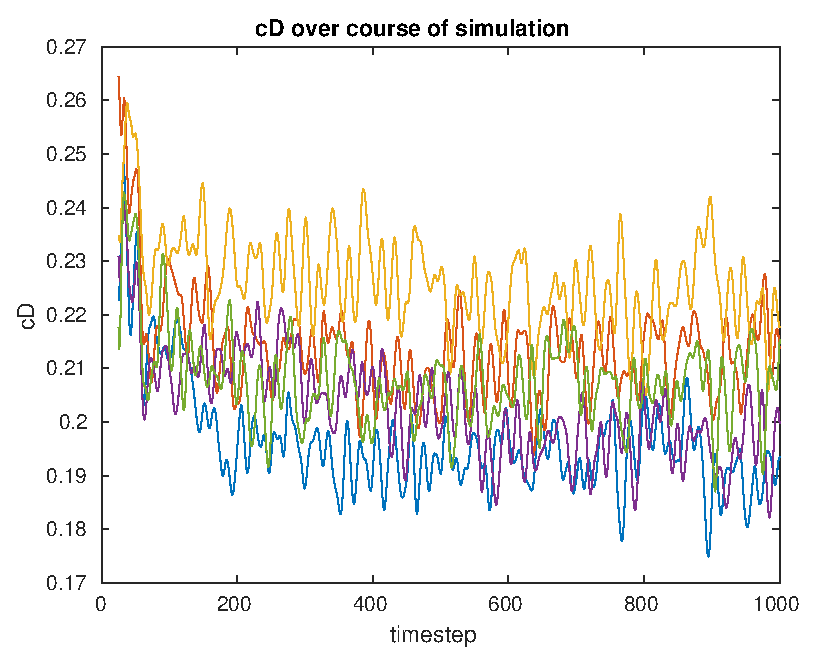
\includegraphics[width=.8\linewidth]{bilder/escooterCDConvergence}
	\caption{Konvergenz}
	\label{fig:escooter_convergence}
\end{figure}

Auch der E-Roller wird zuerst mit snappyHexMesh gemesht, worauf die Fluiddynamiksimulation mit simpleFoam folgt. 
Es wurde wieder der "distance" Modus von snappyHexMesh genutzt um abhängig von der Distanz zum E-Roller Zellen mehr oder weniger zu verfeinern.
In den Openfoam Simulationen stellte sich allerdings heraus, dass die cD-Werte, wie in \cref{fig:escooter_convergence} zu sehen ist, nicht ausreichend konvergieren.
Selbst wenn die nach 1000 simulierten Sekunden ist eine Konvergenz nicht absehbar, im Gegenteil ist vom hundertsten bist zum tausendsten Zeitschritt keine Verbesserung bezüglich der Konvergenz festzustellen.
Auch entsteht keine regelmäßige Oszillation aus der der Mittelwert einfacher ermittelt werden kann.
Stattdessen schwingt der cD-Wert eher unregelmäßig, was die Berechnung eines Fitnesswerts erheblich erschwert.
Das die Simulation nicht konvergiert kann verschiedene Gründe, wie beispielsweise die falsche Parametrisierung der Simulation oder die falsche Auswahl der Simulationsfunktion, haben.
Die Untersuchung und Anpassung von Openfoam zur Behebung dieses Problems sprengt allerdings den Rahmen dieser Arbeit, zur Fitnessberechnung wurden die Simulationen daher mit 1000 Zeitschritten durchgeführt und der cD-Wert über die letzten 900 Zeitschritte gemittelt.
Ergebnisse in der E-Rollerdomäne müssen daher unter Vorbehalt getroffen werden, da die Möglichkeit besteht, dass die Ergebnisse der Openfoam-Simulationen inkorrekt oder zumindest ungenau sind.

\subsubsection{Constraint}

In der E-Roller Domäne existierten einige Constraints. Anders als beim Velomobil konnten diese allerdings durch die Wahl der Repräsentation bereits ausgeschlossen werden.
Zuerst muss das Bauteil einen gewissen Abstand zur Fahrbahn haben, um mit dieser nicht zu kollidieren.
Bauteile, die dies nicht erfüllen, können durch die Wahl der maximalen Deformationstärke ausgeschlossen werden.
Außerdem muss das Bauteil am restlichen E-Roller befestigt werden. Dafür darf die vordere Kante des Bauteils nicht deformiert werden.
Dies kann vermieden werden, indem die Dimensionen der FFD-Box so gewählt werden, dass die vordere Kante nicht in dieser liegt.
Dadurch wird ausgeschlossen, dass diese Kante deformiert wird und der korrekte Anschluss von Bauteil zum Rest des Rollers ist gewährleistet.

\subsubsection{Wahl der Features}

Die Wahl der Features in der E-Roller Domäne ist relativ ähnlich zu der Radkastendomäne.
Statt der Breite ist hier die Höhe beziehungsweise Tiefe des Bauteils interessant.
Als erstes Feature wurde daher die z-Koordinate des tiefsten Punkts des Bauteils gewählt.
Im Gegensatz zum Velomobil kann keine klare Hypothese aufgestellt werden , ob die Höhe des Bauteils mit dessen Effekt auf den Luftwiderstand des E-Rollers korreliert ist.
Zwar ist zu erwarten, dass der Luftwiderstand des Bauteils durch eine höhere Angriffsfläche steigt, es ist aber möglich, dass ein höheres Bauteil die Strömung im hinteren Bereich so weit verbessert, dass insgesamt eine Minderung des Luftwiderstands stattfindet.

Als zweites Feature wurde die x-Koordinate des tiefsten Punktes gewählt.
Effektiv bedeutet das, dass unterschieden wird ob dieser weiter vorne oder hinten liegt.
Auch hierzu ist keine klare Hypothese aufzustellen, ob und wenn ja welchen Effekt die Position des tiefsten Punkts auf die Aerodynamik hat.

\subsubsection{Deformationspunkte}
\begin{figure}[h]
	\centering
	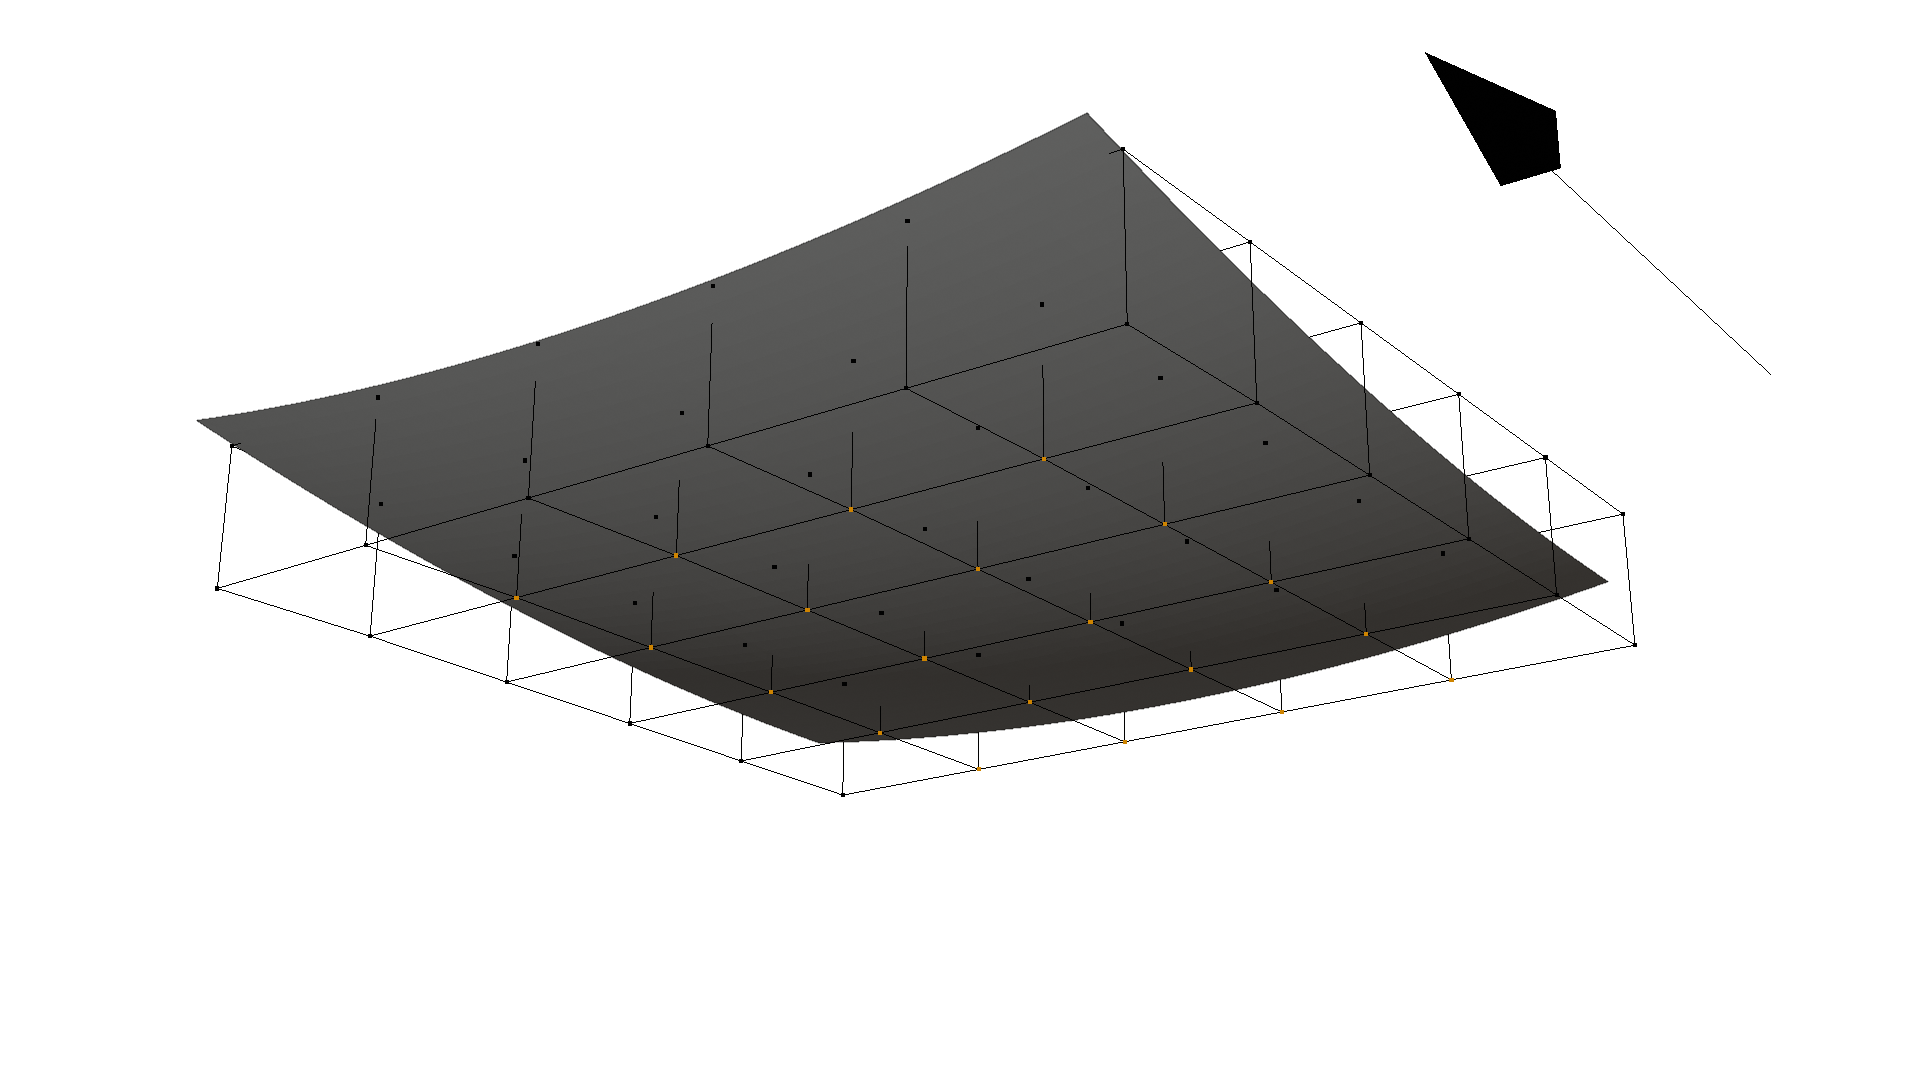
\includegraphics[width=.8\linewidth]{bilder/escooter_deformationPoints}
	\caption{Die FFD-Box und Deformationspunkte des E-Roller-Bauteils. Pfeil zeigt in Fahrtrichtung}
	\label{fig:escooter_deformation}
\end{figure}
Grundsätzlich interessant sind Deformationen des Bauteils nach unten.
In \cref{fig:escooter_deformation} sind die Deformationspunkte dargestellt mit denen das Bauteil deformiert wird.
Da die Vertikale die interessante Dimension ist, werden diese Punkte nur in y-Richtung deformiert.
Dadurch kann eine höherere Anzahl an Deformationspunkten gewählt werden.






